\documentclass{article}
\usepackage[table]{xcolor}
\usepackage{multirow}
\usepackage{mathtools}
\usepackage{caption}
\usepackage{subcaption}
\usepackage{enumitem}
\usepackage{multicol}
\usepackage[toc,page]{appendix}
\usepackage[gen]{eurosym}
\usepackage{tabularx}
\usepackage{epigraph}
\usepackage{textcomp}
\usepackage[english]{babel}
\usepackage[utf8]{inputenc}
\usepackage{amsmath}
\usepackage{amsthm}
\usepackage{amssymb}
\usepackage{hyperref}
\usepackage{csquotes}% Recommended
\usepackage{rotating}
\usepackage[style=numeric]{biblatex}
% \bibliography{<mybibfile>}% ONLY selects .bib file; syntax for version <= 1.1b
\addbibresource{literature.bib}% Syntax for version >= 1.2

\usepackage{graphicx}
\graphicspath{{./images/}}

\usepackage{fancyhdr}
\pagestyle{fancy}
\lhead{}
\chead{}
\rhead{}
\lfoot{}
\cfoot{\thepage}
\rfoot{Property of V-Research}
\renewcommand\headrulewidth{0pt}
\renewcommand\footrulewidth{0pt}

\usepackage[colorinlistoftodos]{todonotes}

\newcommand{\Paragraph}[1]{\smallskip\noindent{\bf #1.}}
\newcommand{\fixnote}[2]{\textbf{\color{red}{FIX}}\footnote{{\bf #1:} #2}}
\newcommand{\fix}[2]{{\color{red} {\bf tofix:} #2}}
% \renewcommand{\fixnote}[2]{}
% \renewcommand{\fix}[2]{}

%colors in tables
\definecolor{abfred}{RGB}{255, 215, 215}
\definecolor{abf-rg-1}{RGB}{251,213,242}
\definecolor{abf-rg-2}{RGB}{243,212,249}
\definecolor{abf-rg-3}{RGB}{213,210,245}
\definecolor{abf-rg-4}{RGB}{208,231,242}
\definecolor{abf-rg-5}{RGB}{206,238,223}
\definecolor{abf-rg-6}{RGB}{205,236,210}
\definecolor{abf-rg-7}{RGB}{211,234,204}
\definecolor{abfgreen}{RGB}{221,232,203}

\definecolor{abforange}{RGB}{255, 245, 206}


\theoremstyle{definition}
\newtheorem{definition}{Definition}[section]
\theoremstyle{corollary}
\newtheorem{corollary}{Corollary}[section]
\theoremstyle{lemma}
\newtheorem{lemma}{Lemma}[section]
\theoremstyle{theorem}
\newtheorem{theorem}{Theorem}[section]
\theoremstyle{theorem}
\newtheorem{example}{Example}

\usepackage{authblk}
\date{}                     %% if you don't need date to appear
\setcounter{Maxaffil}{0}
\renewcommand\Affilfont{\itshape\small}

% for fancy table with rotated column titles
\usepackage{adjustbox}
\newcolumntype{R}[2]{%
    >{\adjustbox{angle=#1,lap=\width-(#2)}\bgroup}%
    l%
    <{\egroup}%
}
\newcommand*\rot{\multicolumn{1}{R{45}{0.01em}}}% no optional argument here, please!
\newcommand*\rota{\multicolumn{1}{R{90}{0.01em}}}% no optional argument here, please!
\def\hb{\hbox to 10.7 cm{}}

% circles
\usepackage{wasysym}
\newcommand{\Tdot}{$\CIRCLE$}
\newcommand{\Thdot}{$\LEFTcircle$}
\newcommand{\Twdot}{$\Circle$}

% formulas
\newcommand{\kframe}{\mathbf{K}}
\newcommand{\bframe}{\mathbf{B_K}}
\newcommand{\possibleworlds}{G}
\newcommand{\modalrelation}{R}
\newcommand{\actualworld}{\omega*}
\newcommand{\world}{\omega}
\newcommand{\World}{\Omega}
\newcommand{\kmodel}{M}
\newcommand{\interpretation}{\sigma}
\newcommand{\knowledgeRegion}{\mathbb{K}}
\newcommand{\knowledge}[1]{\mathbb{K}_{#1}}
\newcommand{\knows}[2]{K_{#1}#2}
\newcommand{\belief}[1]{\mathbb{B}_{#1}}
\newcommand{\believe}[2]{B_{#1}#2}
\newcommand{\beliefRegion}{\mathbb{B}}
\newcommand{\region}{\chi}
\newcommand{\Region}{\mathrm{X}}
\newcommand{\agentuniverse}{\mathcal{A}}
\newcommand{\agent}{a}
\newcommand{\system}{s}
\newcommand{\follang}{\mathcal{L}}
\newcommand{\weakness}{w}
\newcommand{\Weakness}{W}
\newcommand{\vulnerability}{v}
\newcommand{\Vulnerability}{V}
\newcommand{\information}[1]{\mathbb{I}_{#1}}
\newcommand{\informs}[2]{I_{#1}#2}
\newcommand{\informationRegion}{\mathbb{I}}
%ABF
\newcommand{\assertionRegion}{\mathcal{A}}
\newcommand{\behaviorRegion}{\mathcal{B}}
\newcommand{\factRegion}{\mathcal{F}}
\newcommand{\abf}{\assertionRegion,\behaviorRegion,\factRegion}
\newcommand{\abftheory}{\assertionRegion\behaviorRegion\factRegion}
\newcommand{\rassert}[3]{\mathcal{A}_{#1\rightarrow #2}#3}
\newcommand{\lassert}[3]{\mathcal{A}_{#1\leftarrow #2}#3}
\newcommand{\behave}[2]{\mathcal{B}_{#1}#2}
\newcommand{\fact}[2]{\mathcal{F}_{#1}#2}
\newcommand{\asset}[1]{\text{asset}({#1})}
%rcc5
\newcommand{\rcc}{rcc}
\newcommand{\Rcc}[2]{rcc(#1,#2)}
\newcommand{\connects}[2]{C(#1,#2)}
\newcommand{\disconnected}[2]{\neg C(#1,#2)}
\newcommand{\partof}[2]{P(#1,#2)}
\newcommand{\overlaps}[2]{O(#1,#2)}
\newcommand{\eq}[2]{EQ(#1,#2)}
\newcommand{\pp}[2]{PP(#1,#2)}
\newcommand{\po}[2]{PO(#1,#2)}
\newcommand{\ppi}[2]{PPi(#1,#2)}
\newcommand{\dr}[2]{DR(#1,#2)}
\newcommand{\all}[2]{T(#1,#2)}

\newcommand{\abftool}{ABFtool}
\newcommand{\secramod}{V-SecRA}
\newcommand{\designverifmod}{V-DesignVerif}
\newcommand{\atgmod}{V-ATG}

\makeindex 

\begin{document}

\title{On Cybersecurity\\Science and Engineering\footnote{Confidential, restricted to the authors. Property of V-Research}}
\author[1]{Francesco Beltramini}
\author[1]{Marco Rocchetto}
\affil[1]{V-Research, Verona, Italy}

\maketitle

\begin{abstract}
 The objective of this research is to develop of a theory that defines
(all and only) the possible insecurity and security configurations of
any abstract system. The theory is structured upon other theories that 
defines how a component of a system can be abstracted into an agent, defining how
agents can be formalized (both syntactically and semantically) to
describe an abstract system, such as a graph. Some of these theories
(e.g. used for the semantic
definition of the abstract system) are the epistemological definition
of knowledge, the Belief-Desire-Intent and the Assertion-Belief-Fact 
framework of reference, 
mereology, and topological structure. We argue that a mereology is the
most appropriate abstract underlying structure, do to its generality,
for defining the expressiveness of the system abstraction.  Furthermore, a
mereology allows us to define an ontology rather than a taxonomy.  We
also correlate different abstractions of the system to the TRL and the
engineering V-model. 

We implemented a formal theory (of axioms) of a mereotopology, and of
the Region Connection Calculus (RCC3 and RCC5) in a Python program that
uses the Z3 SMT solver. The results show that a single component (i.e.
agent) of an abstract system has a definite number of  different
insecurity configurations (e.g. 53 using RCC5 over a topological
structure) and only 1 secure (i.e. expected) configurations. The
configurations are reported as models satisfying the abstract system
semantics. 

We considered the philosophical definition of truth behind our
approach, rejecting ``proof'' by induction from partial empirical evidences.
Our theory can be applied to system engineering and we show a concrete
application of our theory to the risk assessment of an ad-hoc system.
Finally, we provide a number of ideas to support the engineering of
secure systems (e.g. purely cyber or cyber-physical).

\end{abstract}
\newpage

\section{Introduction}\label{sec:intro}
\epigraph{Humanum est errare}{{\itshape Seneca the Elder}}
The European Commission states in\autocite{EU2019market} that: ``Cybersecurity
is one of the priority areas [\ldots] of the Commission initiative on ICT
Standards, which is part of the Digitising European
Industry\autocite{EU2019standard} strategy launched on 19 April 2016.  The aim
is to identify the essential ICT standards and present measures to accelerate
their development in support of digital innovations across the economy''. The
same document (i.e.\autocite{EU2019market}) states that ``The EU will invest up
to \euro450 million [\ldots], under its research and innovation programme
Horizon 2020''. The EU, in 2016 published a press release\autocite{EU2016press}
in which they present a strategy to invest \euro1.8 \emph{billion} to
``increase measures to address cyber threats''. The EU is not the only investor
in cybersecurity, most of the developed countries and several companies are
investing enormous amount of money towards various aspects of cybersecurity
(e.g. The US vulnerability databases\autocite{NIST2020NVD} maintained by the
National Institute of Standards and Technologies, i.e. NIST, of the US
Department of Commerce).

The cybersecurity industry is growing fast, e.g. as reported
in\autocite{Nasdaq2018market}. For example, in\autocite{Forbes2017market},
published by the Forbes, is stated that \euro5.3 billion of funding where
poured by venture capitalist into cybersecurity companies in 2018. The Forbes,
in the same article, also highlights another peculiar (as seemly contradictory)
trend: ``[\ldots] during the same time period, the number of cybersecurity
breaches increased exponentially''. The data reported by the NIST 
through the official CPE (Common Platform Enumeration) Dictionary Statistics 
on the NVD websites in \autocite{NIST2020CPEstatistics}, show that in 2016 the
number of reported vulnerabilities reported where around $~6000$ while in 2019
the number of vulnerabilities was above $16000$.  The scientific community also
reports seemingly unjustifiable findings.  In fact, in\autocite{Herley2009so}, Cormac Herley
(Microsoft Research) shows how basic cybersecurity principles (such as the
confidentiality benefit over the clear text for passwords typed into forms,
e.g. for logins in websites) are not fully understood or shared between the
cybersecurity research community\autocite{Nielsen2009stop}.  The lack of
understanding of basic security principle, the inverse proportionality between
investments in cybersecurity and the number of reported vulnerabilities year
after year, can be linked to the lack of a foundational theory on
cybersecurity, as already highlighted by Cormac Herley
in\autocite{Herley2016unfalsifiability}. 

Another way of looking at the same problem is by analyzing the different
definitions of security with respect to the scientific method of enquiry
applied to get to the definition itself. In the following we categorize the
related work into three categories, as defined by Sextus Empiricus in
\autocite{Empiricus1990Pyrrhonism}.  To the best of our knowledge, there is no
evidence that this categorization isn't complete.  ``The natural result of any
investigation is that the investigators either discover the object of search or
deny that it is discoverable and confess it to be in-apprehensible or persist
in their search. [\ldots] This is probably
why''\autocite{Empiricus1990Pyrrhonism}: 
\begin{itemize}
	\item The \emph{dogmatists} ``have claimed to have discovered the truth'' on what cybersecurity is
		\begin{itemize}
			\item Wikipedia defines cybersecurity in
				\autocite{wiki-cybersecurity} as the protection
				of computer systems and networks from the theft
				of or damage to their hardware, software, or
				electronic data, as well as from the disruption
				or misdirection of the services they provide
		\end{itemize}
	\item The \emph{academics} ``have asserted that it cannot be apprehended''
		\begin{itemize}
			\item Eugene H. Spafford, Professor at Purdue
				University, defines cybersecurity as follow.
				``The only truly secure system is one that is
				powered off, cast in a block of concrete and
				sealed in a lead-lined room with armed guards —
				and even then I have my doubts.''
				\autocite{Spafford2019Quotes}
		\end{itemize}
	\item The \emph{skeptics} ``go on inquiring''
		\begin{itemize}
			\item Cormac Herley reaches the conclusion that
				cybersecurity has no definition. ``There is an
				inherent asymmetry in computer security: things
				can be declared insecure by observation, but
				not the reverse. There is no test that allows
				us to declare an arbitrary system or technique
				secure. This implies that claims of necessary
				conditions for security are unfalsifiable. ''
				\autocite{Herley2016unfalsifiability}
		\end{itemize}
\end{itemize}

The method applied in our line of research follows what the scientific method
mandate. We start by detailing the problem statement by reporting the state of
the art in Section~\ref{sec:problem}, we formulate (inductively)\footnote{``So,
whenever they argue ``Every man is an animal and Socrates is a man; therefore
Socrates is an animal,'' proposing to deduce from the universal proposition
``every man is an animal'' the particular proposition ``Socrates therefore is
an animal,'' which in fact goes (as we have mentioned) to enstablish by way of
induction the universal proposition, the fall into the error of circular
reasoning, since they are enstablishing the universal proposition inductively
by means of each of the particulars and deducing the particular
proposition from the universal syllogistically.'' Sextus Empiricus, Outlines of
Pyrrhonism II-195 \autocite{Empiricus1990Pyrrhonism}} hypothesis based on our
review (Section~\ref{sec:glossary}) which we use to propose a theory in
Section~\ref{sec:theory} that apply to a abstract and standard (i.e. based on
standards) secure process development lifecycle based on requirement
engineering in Section~\ref{sec:engineering} (with an ad-hoc running example,
based on the SWaT testbed \autocite{Mathur2016swat}).  We propose a tool for
the risk assessment of a design based on our theory in Section~\ref{sec:tool}.
Finally, in Section~\ref{sec:conclusion} we conclude the paper.


\section{Problem Statement}\label{sec:problem}
Before going into the details of the literature review, we show that the lack
of agreement on what security is can actually be found in the literature, and
can be categorized with respect to the method of enquiry.  In the following, we
provide three examples based on the categorization provided by Sextus Empiricus
in \autocite{Empiricus1990Pyrrhonism}, since it appear to us to be
comprehensive. ``The natural result of any investigation is that the
investigators either discover the object of search or deny that it is
discoverable and confess it to be in-apprehensible or persist in their search.
[\ldots] This is probably why''\autocite{Empiricus1990Pyrrhonism}: 
\begin{itemize}
	\item The \emph{dogmatists} ``have claimed to have discovered the truth''
		\begin{itemize}
			\item Wikipedia defines cybersecurity in
				\autocite{wiki-cybersecurity} as the protection
				of computer systems and networks from the theft
				of or damage to their hardware, software, or
				electronic data, as well as from the disruption
				or misdirection of the services they provide.
		\end{itemize}
	\item The \emph{academics} ``have asserted that it cannot be apprehended''
		\begin{itemize}
			\item Eugene H. Spafford, Professor at Purdue
				University, defines cybersecurity as follow.
				``The only truly secure system is one that is
				powered off, cast in a block of concrete and
				sealed in a lead-lined room with armed guards —
				and even then I have my doubts.''
				\autocite{Spafford2019Quotes}
		\end{itemize}
	\item The \emph{skeptics} ``go on inquiring''
		\begin{itemize}
			\item Cormac Herley reaches the conclusion that
				cybersecurity has no definition. ``There is an
				inherent asymmetry in computer security: things
				can be declared insecure by observation, but
				not the reverse. There is no test that allows
				us to declare an arbitrary system or technique
				secure. This implies that claims of necessary
				conditions for security are unfalsifiable. ''
				\autocite{Herley2016unfalsifiability}. Therefore, we propose our investigation.
		\end{itemize}
\end{itemize}

\begin{figure}[t]
	\centering
	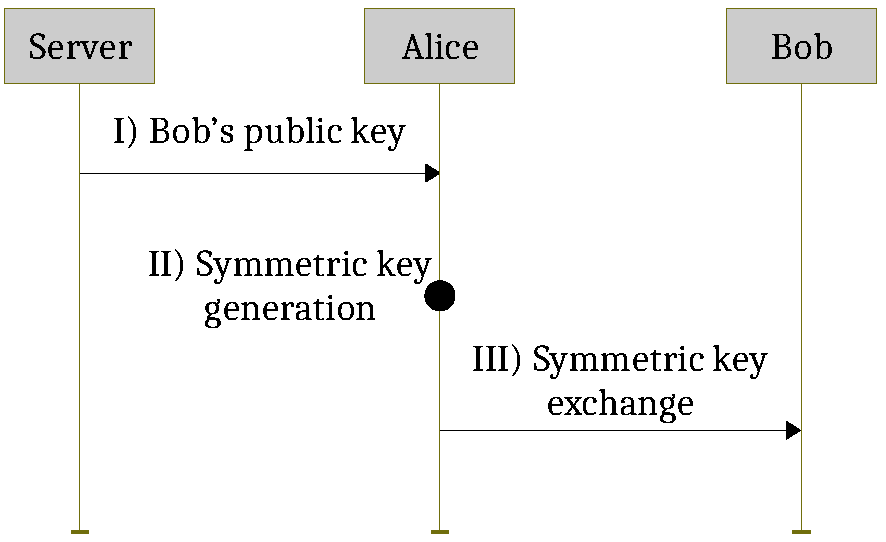
\includegraphics[width=.6\textwidth]{protocol-example.pdf}
	\caption{Abstraction of an ad-hoc esemplificative protocol execution}
	\label{fig:protocol-example}
\end{figure}

In\autocite{Herley2016unfalsifiability}, Cormac Herley explores what he calls
``an asymmetry in computer security'', which he defines as follows: ``Things
can be declared insecure by observation, but not the reverse. There is no
observation that allows us to declare an arbitrary system or technique
secure''. Herley then uses this argument to show that ``claims that any measure
is necessary for security are empirically unfalsifiable''. Given that, any
theory which is not falsifiable by an empirical experiment is well
known\footnote{``A theory which is not refutable by any conceivable event is
nonscientific. Irrefutability is not a virtue of a theory (as people often
think) but a vice.'' -- Karl Popper, Conjectures and
Refutations\autocite{popper1962conjectures}} to be nonscientific (i.e.
unfalsifiability is a fallacy of a theory), Herley concludes that there is no
scientific theory on cybersecurity; which means that cybersecurity lays in the
realm of pseudo-sciences\autocite{Herley2016usenixvideo}.  Herley, e.g.
in\autocite{Herley2017justifying}, discusses the implications of a
nonscientific approach to cybersecurity, and highlights the tremendous impact on
all the scientific research and engineering of systems; leading often to
terrorism and wars, and wasting of resources in useless protections or
overspending.  While the criticism is investigated
in\autocite{Herley2016unfalsifiability}, no solution is provided.  On the
contrary, the goal of this work \emph{is} to lay the foundations of a
scientific cybersecurity theory. Furthermore, in Section~\ref{sec:sicurezza},
we consider the problem raised by Herley not confined to ``computer security''
but to any abstract system (so that our theory may hold for any sound
implementation such as networks, mechanical, cyber, or cyber-physical system,
or even a single computer or a single device such as an hard-drive).  There is
also an apparent inconsistency in\autocite{Herley2016unfalsifiability} that we
seek to clarify before following (as we agree) the scientific path draw by
Herley: cybersecurity is defined as an abstract property in many formal
approaches to the investigation of the security of systems, and the security of the design of a
formally verified protocol is indeed falsifiable (against the security properties verified).  For example, in the protocol
verification community, security is often defined as a formalization of the
high-level properties confidentiality, integrity, and availability. The problem
in such approaches is not the definition of what cybersecurity is but 
the generality of the results, since they takle a specific step (and not the first) of the engineering process (of system).
Therefore, the theories underlying the verification are based on 
assumptions which non-evidently apply to a general security theory.
As an example, the so called Dolev-Yao attacker model\footnote{For the sake of
simplicity, the Dolev-Yao attacker can be considered as an abstraction of an
active attacker who controls the network but cannot break
cryptography.}\autocite{Dolev1983security}
that only applies to specific instances (often called scenarios) and
abstraction of the protocol. This, in turn, creates a false sense of security
since requires non-justifiable assumptions on the abstraction of the system of which security
is verified. More specifically, for the formal security verification of the system
in Figure~\ref{fig:protocol-example}, a formalized scenario needs to be defined
by a modeler who chooses (among others): (i) a scope of the formalization (e.g.
excluding the server that distributes the public key is often done when
verifying the security of authentication protocols), (ii) the number of
sessions (even tough some approaches do reason on an infinite number of
sessions such as\autocite{Escobar2007maudenpa}), (iii) honesty/dishonesty of
the peers (e.g.  in the ASLan++ language\autocite{Oheimb2010aslan++}), and (iv)
the abstraction of the cryptographic primitives (e.g.  ProVerif vs
CryptoVerif\autocite{Blanchet2017symbolic}).  While many tools and theories
improves the issues we discussed, there is no agreement on which should be
the definitive approach if any and, more importantly, some of the choices made by the modelers/engineers using those formal apporaches may
completely change the results of the formal verification of the system (an interesting example on how difficult it is to 
even just compare the approaches is given in \autocite{Cremers2009comparing}). For
example, under the perfect cryptography assumption\footnote{As defined
in\autocite{Rocchetto2016cpdy}: ``In the so called perfect cryptography
assumption, the security encryption scheme is suppose to be perfect, without
any exploitable flaw, and so the only way for the attacker to decrypt a message
is by using the proper key. That assumption is widely accepted in the security
protocol community, and most of the formal reasoning tools for the analysis of
security protocols abstract away the mathematical and implementation details of
the encryption
scheme\autocite{Turuani2006clatse,Basin2005ofmc,Armando2016satmc,Rocchetto2017interpolation}''}
and assuming that no violation to any security property is done after message
I); in Figure~\ref{fig:protocol-example}, the freedom of choosing the scope
determines that the flaws related to the dishonest impersonation of the Server
may or may not be considered in the verification process.  This choice has
tremendous impact on the focus and findings of the verification of the security
of the protocol.  While this may seem to turn upon minutiae and foreseeable,
this highlights the false sense of security that may derive from a
non-falsifiable theory of system security\footnote{``To the superficial
observer, the analysis of these forms seems to turn upon minutiae. It does in
fact deal with minutiae, but they are of the same order as those dealt with in
microscopic anatomy.'' -- Karl Marx, Capital Volume 1, 1867}.

\subsection{Terminology: Safety or Security}\label{sec:sicurezza}
In most of the natural languages, and in Italian too, the concepts of safety
and security are not syntactically differentiated and both terms (safety and
security) are expressed by the same word, e.g. sicurezza in Italian.  A
semantic distinction between safety and security is correlated to a
belief\footnote{A belief has to be intended as a proposition which is supposed
to be true by the majority of people in our society, without a scientific
underlying theory but based on partial empirical evidences or inductive reasoning based on partial empirical evidences.} that
safety deals with \emph{accidents} (i.e. an unfortunate incident) posed by the
natural environment (e.g. natural events such as wearing of hardware
components) while security deals with \emph{incidents} posed by mankind (e.g.
attackers and bugs).  The fundamental difference between nature and mankind (and,
in turn, between safety and cybersecurity) is believed to be on the different
intents\footnote{``The belief–desire–intention software model (BDI) is a
software model developed for programming intelligent
agents.''\autocite{wiki-bdi}. In the BDI model, the intents represents the
deliberative state of an agent which determines the choice of that agent on
what to do.} (accidents are unfortunate while incidents are not) of the causes
that generates a threat; namely, nature is believed not to have malicious
intents (but unfortunate causes-effects) while threats generated by mankind are
believed to be malicious\footnote{Of course, logical flaws or bugs may be
introduced by other means (e.g. ignorance) without explicit malicious intents,
but the exploitation of those flaws is considered (for now, and detailed
afterwards in the article) malicious, and then we consider any vulnerability to
be malicious even if due to the lack of skills.}.
An overview on the aforementioned aspects of safety and security is depicted in
Figure~\ref{fig:safety-security} and is used as a baseline for a definition of
the terms that structure our current understanding of safety and security. 
\begin{itemize}
	\item \emph{Mankind} ``refers collectively to humans''
\autocite{wiki-mankind}, while the concept of \emph{Nature} is
		related ``to the intrinsic characteristics that plants,
		animals, and other features of the world develop of their own
		accord'' (e.g. the physical universe)\autocite{wiki-nature}. 
		\begin{itemize}
			\item So far, we have used several terms to refer to an
				\emph{attacker}, i.e. threat agent or threat source,
				considering those terms to be semantically
				equivalent.  This ``shallowness'' has raised form the
				necessity of properly citing the different sources, but,
				in the reminder of this paper, we consider the
				Causality principle to be the \emph{threat
				source}, Nature or Mankind to be the
				\emph{threat agents} and an \emph{attacker} as
				a specific malicious threat agent which materializes a
				threat.
		\end{itemize}
	\item \emph{Vulnerability}\footnote{The term vulnerability is not
		present in the Encyclopedia of Cryptography and Security, while
		it is used in 12 entries (such as in the definition of
		``penetration testing''\autocite{caddy2005pentest})
		highlighting how commonly this word is used without a proper
		supporting semantics.}, as defined in\autocite{cnssi20104009}
		(and adopted in\autocite{nist2013800-53}), is ``weakness in an
		information system, system security procedures, internal
		controls, or implementation that could be exploited by a threat
		source''. On the one hand, the definition is broad to enclose
		as much causes (that generates a vulnerability) as possible; on
		the other hand, it derives from empirical evidences (which
		should be considered beliefs\footnote{``For this view, that
		\emph{That Which Is Not} exists, can never predominate. You
		must debar your thought from this way of search, nor let
		ordinary experience in its variety force you along this way,
		(namely, that of allowing) the eye, sightless as it is, and the
		ear, full of sound, and the tongue, to rule; but (you must)
		judge by means of the Reason (Logos) the much-contested proof
		which is expounded by me.'' -- Parmenides of Elea, On Nature
		(circa 500 B.C.), fragments B7.1–8.2
		\autocite{Hakim2016philosophy}} since they are partial results in nature) 
		%while a vulnerability should
		%be defined in a way that is empirically falsifiable. This means
		%that 
		On the other hand, the term vulnerability should have a complete and sound
		definition, so that no other causes (e.g.  other sources) but
		the ones in the definition are responsible for a vulnerability.
		Furthermore, the term ``threat sources'' used in the definition
		in\autocite{cnssi20104009} may be identified with both Nature
		and Mankind, not differentiating between safety and security.
\end{itemize}

\begin{figure}[t]
	\centering
	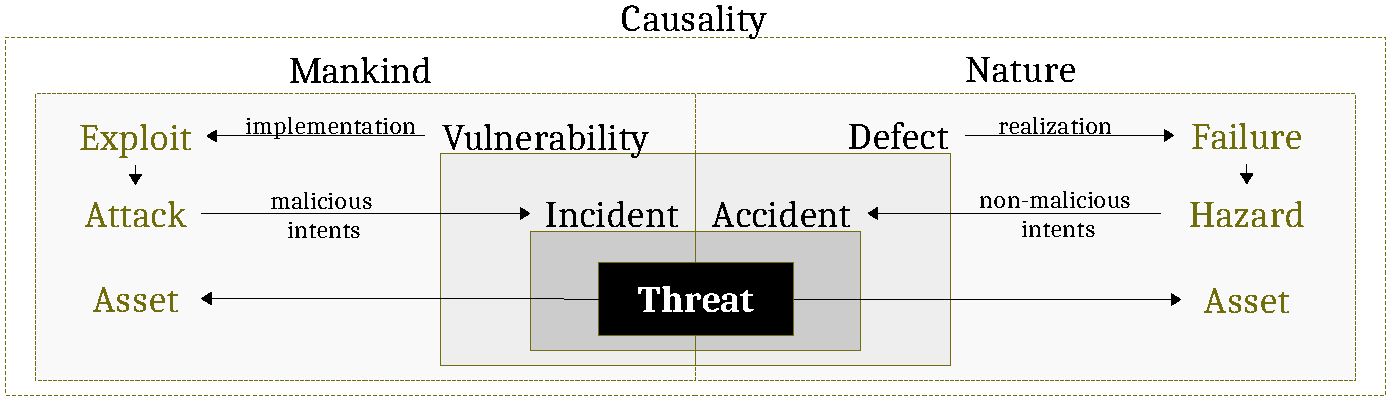
\includegraphics[width=\textwidth]{safety-security.pdf}
	\caption{Overview of keywords related to security and safety}
	\label{fig:safety-security}
\end{figure}

Most of the safety-preserving principles in the field of engineering of
safety-critical cyber-physical systems (such as elevators and aircraft), upon
which safety requirements are defined (e.g. in standards such as the IEC 61508 or 61511\autocite{IEC201761511}), 
are based on empirical tests and measurements (therefore should be considered hypothesis and not definitions). While reasoning by
induction based on the empirical observation should be avoided, since it may
easily lead to false beliefs, this approach is
often justified by the supposed impossibility of defining a theory that
correctly predicts failures.
%which, in turn, pose hazards to a system. 
To the best of our knowledge, and supported by\autocite{Herley2016unfalsifiability}, %the
there is no scientific theory that defines what a secure system is.
%correlation between predictability of environment and believed unpredictability
%of attackers has not been correlated to a theory on cybersecurity. 
Therefore, 
(inductive\footnote{``So, whenever they argue ``Every man is an
animal and Socrates is a man; therefore Socrates is an animal,'' proposing to
deduce from the universal proposition ``every man is an animal'' the particular
proposition ``Socrates therefore is an animal,'' which in fact goes (as we have
mentioned) to enstablish by way of induction the universal proposition, the
fall into the error of circular reasoning, since they are enstablishing the
universal proposition inductively by means of each of the particulars and
deducing the particular proposition from the universal syllogistically.''
Sextus Empiricus, Outlines of Pyrrhonism II-195
\autocite{Empiricus1990Pyrrhonism}})
research efforts in
predicting malicious effects are accepted (and published) in scientific
conferences (e.g.~\autocite{Rocchetto2014CSRF}). A failure of a wire due to
environment (e.g. due to humidity, dust, heat \&c) is defined from empirical
evidences and processes have been standardized to test qualities of hardware components.
This process completely breaks down when a malicious environment (i.e. an attacker)
is considered instead of the (supposedly honest and predictable)
natural environment. Therefore, the same approach that is in use for safety,
seems not to be applicable for security (e.g. for security testing).

Going back to Figure~\ref{fig:safety-security}, a vulnerability does not
necessarily become a threat for the system, unless exploited ``through a
channel that allows the violation of the security policy
[\ldots]''\autocite{cnssi20104009}. For example, a software or procedure that takes
advantage of the vulnerability causing an \emph{attack} to the system may
result in several correlated incidents and threats.  The process of
exploitation of a defect as a vulnerability is reported in
Figure~\ref{fig:safety-security} such that the difference between exploit and failure,
and attack and accident is to be found just in the maliciousness of the intents
that causes this process (i.e. excluding the intent, the terms are just syntactic transformation from a vulnerability to defect, from
accident to incident). In the following, we conclude the informal definition of
the terms that we used in this section and in Figure~\ref{fig:safety-security}.

\begin{itemize}
	\item \emph{Causality} refers to the causality principle; defined
		in\autocite{Spirkin1983Dialectical} as ``Causality is a genetic
		connection of phenomena through which one thing (the cause)
		under certain conditions gives rise to, causes something else
		(the effect). The essence of causality is the generation and
		determination of one phenomenon by another. In this respect,
		causality differs from various other kinds of connection, for
		example, the simple temporal sequence of phenomena, of the
		regularities of accompanying processes''.
	\item An \emph{Exploit}\footnote{We note that the term exploit is only
		used as a verb in\autocite{ISO2009information}} ``[\ldots]
		(from the English verb to exploit, meaning to use something to
		one’s own advantage) is a piece of software, a chunk of data,
		or a sequence of commands that takes advantage of a bug or
		vulnerability to cause unintended or unanticipated behavior to
		occur on computer software, hardware, or something electronic
		(usually computerized).''\autocite{wiki-exploit}.
	\item An \emph{Attack}, as defined by the International Standard
		ISO/IEC 27000 is an ``attempt to destroy, expose, alter,
		disable, steal or gain unauthorized access to or make
		unauthorized use of an asset''; where an \emph{Asset} is
		``anything that has value to the organization''. We note that for
		the purpose of this article, we do not want to focus on a specific
		organization or business to define asset but, in general, on any 
		abstract organization (e.g. a company or a society).
		We do not consider ethical hackers as attacking a system. 
		In fact, we consider the term \emph{hack} as
		non-malicious (as, e.g. in \autocite{Stallman2002hacker}).
	\item A \emph{Threat}, as defined in\autocite{cnssi20104009}, is ``Any
		circumstance or event with the potential to adversely impact
		organizational operations (including mission, functions, image,
		or reputation), organizational assets, individuals, other
		organizations, or the Nation through an information system via
		unauthorized access, destruction, disclosure, modification of
		information, and/or denial of service''.
	\item \emph{Defect}, ``anything that renders the product not reasonably
		safe''\autocite{Robinson2019writing} (i.e. a characteristic of
		an object which hinders its proper usability).
	\item \emph{Failure}, as defined in\autocite{Merriam2020failure} as ``a state of
		inability to perform a normal function''. The term is
		structured and detailed in
		\autocite{cnssi20104009,iet2017glossary} but relying on an
		abstract notion of failure without a specific definition.
	\item \emph{Hazard}, ``a potential source of
		harm''\autocite{iet2017glossary}.
\end{itemize}

Our literature review shows that most of the definitions relates insecurity to
dis-honesty (also called maliciousness or adversarial) of an agent (often
called adversary or attacker). This, however, just moves the problem of
defining what cybersecurity is as the problem of defining what an dishonest
agent can or cannot do in a system\footnote{where an agent is any virtual or
physical entity of the system or using the system (e.g. a device, a software,
or a human being) and dishonesty is not necessarily related to malicious
motivation but also to incompetence or lack of skills.}
As in the Dolev-Yao theory, we may correlate ``being dishonest'' to ``not
following the intended behavior/rules''.  In the case of a generic system, a
dishonest agent is, therefore, any agent that doesn't follow the intended
behavior (or functionality or logic) of the system.  Given the generality of
the definition, and its high level of abstraction, we may
conclude that the hypothesis seems evident. For example, a software can be
considered an agent of the system and whenever it has a bug, it can be
exploited causing an Incident. However, this hypothesis has lead to the
un-testable conclusion that the dishonest behaviors of agents cannot be defined
in general (e.g. due to the heterogeneity of agents and systems) 
and that huge repository of dishonest behaviors should be kept as
definition, such as CWE\autocite{MITRE2020CWEresearch}, CVE\autocite{CVE},
CAPEC\autocite{MITRE2020CAPEC}, NVD\autocite{NIST2020NVD};
or that dishonesty of an agent with respect to a security protocol should be
defined as a number of predefined actions as in
\autocite{Turuani2006clatse,Basin2005ofmc,Armando2016satmc,Rocchetto2017interpolation}
(to name a few). 


\section{Glossary -- A Formalization}\label{sec:glossary}
We now define a formalizations of the concepts described in
Section~\ref{sec:problem} and depicted in Figure~\ref{fig:safety-security}. We
base our formalization on first order logic (FOL) with the standard
truth-value semantics. The choice of this logic is required by the 
semantics of the concepts formalized afterwards in this section. 

We consider a first-order language $\follang$ over a
signature $\Sigma_P$ where $P,P',\ldots,P^n$ represent terms, and
$\varphi,\varphi',\ldots,\varphi^n$ represent formulas.
The syntax is defined as follows.
\begin{displaymath}
	\varphi := P~|~\neg\varphi~|~\varphi\wedge\varphi~|~\varphi\vee\varphi~|~\varphi\Rightarrow\varphi'~|~\forall P.~\varphi~|~\exists P.~\varphi
\end{displaymath}
where $\wedge$, $\neg$, $\vee$, and $\Rightarrow$ are connectives representing
conjunction, negation, disjunction, and (material) implication respectively; while
$\forall$ and $\exists$ represent the standard universal and existential
quantifiers (resp.). Finally, the symbol ``$.$'' is just syntactic sugar. 
We consider $\interpretation\subset\Phi\times\{\top,\bot\}$ as the interpretation
function, where $\Phi$ is any collection of sentences in $\follang$ 
and $\top$ and $\bot$ represent the concepts of ``Tautology/True''
and ``Contradiction/False'' respectively.

Following Figure~\ref{fig:safety-security}, we start by formalizing the outermost term: Causality.

\subsubsection{Causality Principle}\label{sec:causality}
We formalize the Causality Principle starting from a K modal
logic\autocite{Garson2018modal} (i.e. without restrictions on the causality
relation between worlds). The standard definition of K modal logic is given in
Definition~\ref{def:modallogic} in terms of an interpretation function (which
we named $\sigma$ with a slight abuse of notation) defined in
Definition~\ref{def:modalinterpretation}. 
\begin{definition}{\bf K Modal Logic --}\label{def:modallogic}
A K-frame is a frame $ \kframe=\langle \possibleworlds,\modalrelation \rangle $
	in the K modal logic where $ \modalrelation $ is the binary relation
	(i.e. a set of ordered pairs) between possible worlds
	$\modalrelation\subseteq\possibleworlds\times\possibleworlds$, where
	$\possibleworlds$ represents the possible worlds, and
	$\possibleworlds\neq\emptyset$. An actual world
	$\actualworld\in\possibleworlds$ is assumed. For any proposition $P$,
	an interpretation function $\interpretation(\world,P)$ returns the
	truth value of $P$; e.g. $\interpretation(\world,P)=\top$ means that
	$P$ holds in $\world$. A model is defined as the tuple
	$\kmodel=\langle\possibleworlds,\modalrelation,\interpretation\rangle$.
\end{definition}

\begin{definition}{\bf Causality as K Modal Interpretation Function --}\label{def:modalinterpretation}
	Causality is (recursively) defined as the modal interpretation function $\interpretation$, as follows. 
	\begin{enumerate}[noitemsep]
		\item[$(\interpretation0)$] if $\interpretation(\world,P)=\top$ then $\world\models P$
		\item[$(\interpretation1)$] $\world\models\neg P$ iff $\world\not\models P$
		\item[$(\interpretation2)$] $\world\models P \wedge Q$ iff $\world\models P$ and $\world\models Q$
		\item[$(\interpretation3)$] $\world\models\Box P$ iff for any world $\world'\in\possibleworlds$ if $\world \modalrelation\world'$ then $\world'\models P$
		\item[$(\interpretation4)$] $\world\models\Diamond P$ iff there exists a set of worlds $\World'\subset\possibleworlds$ such that for any $\world'\in\World'$, if $\world\modalrelation\world'$ then $\world'\models P$
		\item[$(\interpretation5)$] $\models P$ iff $\actualworld\models P$
	\end{enumerate}
	where truth is defined as necessary with $\Box$ and possible with $\Diamond$.
\end{definition}

%\begin{definition}{\bf Causality --}\label{def:causality}
%	The Causality principle is defined over a K Modal Logic (i.e. without
%	restrictions on the causality relation between worlds) as in
%	Definition~\ref{def:modallogic}, with the standard interpretation
%	function defined in~\ref{def:modalinterpretation}
%\end{definition}

The causality principle has been defined in its
generic form. In fact, the accessibility relation $\modalrelation$ is free from
any axiomatic restriction (e.g. it's not reflexive nor anti-reflexive).  
We will focus in Section~\ref{sec:process} (for our tests) on 
the application of our theory to CPS system engineering.
More detailed case studies (i.e. \fix{mr}{a CPS as a smart power-grid}) 
will be defined in Section~\ref{sec:prototest}, where
the accessibility relation defines in details how the system itself evolves, due to causal relation 
(i.e. by restricting the causality principle only to those cause-effect that defines
the system). Therefore, the definition of $\modalrelation$
will be specialized in a more strict way based on the application domains and case study.

We note that we have defined the
Causality principle without considering it a \emph{threat source} since 
we lack the concept of intent and maliciousness. Similarly, in the 
next sections we won't discriminate between Nature and Mankind until we introduce 
the concepts of maliciousness in Section~\ref{sec:theory} 
and then formally define a threat agent
in the same section.

\subsubsection{Agents: Mankind and Nature}\label{sec:mankind-nature}
\begin{table}[t]
\centering
\setlength{\tabcolsep}{3.5pt}
\renewcommand{\arraystretch}{1}
\scriptsize
\caption{RCC3, RCC5, and RCC8 relations between Regions $X$, $Y$ and $Z$ ~\label{tab:rcc358}~\label{tab:rcc}}
\begin{tabular}{ccclll} 
\rota{\textbf{RCC3}}&\rota{\textbf{RCC5}}&\rota{\textbf{RCC8}}&\textbf{Name} & \textbf{Notation} & \textbf{Definition} \\
\hline
&&&Connects with 			& $\mathit{C}(\mathit{X},\mathit{Y})$ 		& $\mathit{X}\subseteq \mathit{Y}$ \\
&&&Disconnected from		& $\neg \mathit{C}(\mathit{X},\mathit{Y})$		& $\mathit{X}\not\subseteq \mathit{Y}$\\
&&&Part of				& $\mathit{P}(\mathit{X},\mathit{Y})$		& $\forall \mathit{Z} ~\mathit{C}(\mathit{Z},\mathit{X}) \rightarrow \mathit{C}(\mathit{Z},\mathit{Y})$\\
&&&Overlaps			& $\mathit{O}(\mathit{X},\mathit{Y})$		& $\exists \mathit{Z} ~\mathit{P}(\mathit{Z},\mathit{X})\wedge \mathit{P}(\mathit{Z},\mathit{Y})$\\
\Tdot&&&  \textbf{Overlaps Not Equal} 	& $\mathit{ONE}(\mathit{X},\mathit{Y})$		& $\mathit{O}(\mathit{X},\mathit{Y}) \land \neg \mathit{EQ}(\mathit{X},\mathit{Y})$ \\
\Tdot&\Tdot&\Tdot& \textbf{Equal to} 		& $\mathit{EQ}(\mathit{X},\mathit{Y})$  		& $\mathit{P}(\mathit{X},\mathit{Y}) \wedge \mathit{P}(\mathit{Y},\mathit{X})$\\
\Tdot&\Tdot&\Tdot& \textbf{DiscRete from} 		& $\mathit{DR}(\mathit{X},\mathit{Y})$		& $\neg \mathit{O}(\mathit{X},\mathit{Y})$\\
&\Tdot&\Tdot&\textbf{Partial-Overlap}	& $\mathit{PO}(\mathit{X},\mathit{Y})$ 		& $\mathit{O}(\mathit{X},\mathit{Y})\wedge \neg \mathit{P}(\mathit{X},\mathit{Y}) \wedge \neg \mathit{P}(\mathit{Y},\mathit{X})$\\ 
&\Tdot&&\textbf{Proper-Part-of} 	& $\mathit{PP}(\mathit{X},\mathit{Y})$ 		& $\mathit{P}(\mathit{X},\mathit{Y})\wedge \neg \mathit{P}(\mathit{Y},\mathit{X})$\\ 
	&\Tdot&&\textbf{Proper-Part-of-\textit{\textbf{i}}nverse} & $\mathit{PPi}(\mathit{X},\mathit{Y})$ 		& $\mathit{P}(\mathit{Y},\mathit{X}) \wedge \neg \mathit{P}(\mathit{X},\mathit{Y})$\\
&&\Tdot&\textbf{Externally Connected} 	& $\mathit{EC}(\mathit{X},\mathit{Y})$ 		& $\mathit{C}(\mathit{X},\mathit{Y}) \wedge \neg\mathit{O}(\mathit{X},\mathit{Y})$\\ 
&&\Tdot&\textbf{Tangential PP} 	& $\mathit{TPP}(\mathit{X},\mathit{Y})$ 		& $\mathit{PP}(\mathit{X},\mathit{Y})\wedge\exists\mathit{Z}~[\mathit{EC}(\mathit{Z},\mathit{X}),\mathit{EC}(\mathit{Z},\mathit{Y})]$\\ 
&&\Tdot&\textbf{Tangential PPi} 	& $\mathit{TPPi}(\mathit{X},\mathit{Y})$ 		& $\mathit{TPP}(\mathit{Y},\mathit{X})$\\ 
&&\Tdot&\textbf{Non-Tangential PP} 	& $\mathit{NTPP}(\mathit{X},\mathit{Y})$ 		& $\mathit{PP}(\mathit{X},\mathit{Y})\wedge\neg\exists\mathit{Z}~[\mathit{EC}(\mathit{Z},\mathit{X}),\mathit{EC}(\mathit{Z},\mathit{Y})]$\\ 
&&\Tdot&\textbf{Non-Tangential PPi} 	& $\mathit{NTPPi}(\mathit{X},\mathit{Y})$ 		& $\mathit{NTPP}(\mathit{Y},\mathit{X})$\\ 
\end{tabular}
\end{table}

Mankind and Nature are defined in Section~\ref{sec:problem} as two abstract
agents, both as collections (i.e. an abstract type that does not imply a
specific implementation) of their sub-agents (i.e. humans for Mankind and
plants, animals, \&c.  for Nature). Similarly to\autocite{Santaca2016abf}, 
we define Mankind and Nature, and any
other agent in the reminder of this article, as a meronomy (an hierarchy of
Part-Whole relations) based on a standard definition of mereology, i.e. based
on the definition of Parthood relation between \emph{Parts}.  
However, shall 
consider different types of Part; so, we extend the mereology to a
mereo-topology\autocite{Smith1996mereotopology,Varzi1994mereotopology,Rachavelpula2017mereotopology},
to increase the number of different types considered and to generalize the relations between Parts (as
in Table~\ref{tab:rcc358}).
For the sake of readability, we use the term \emph{Region} both to refer to a
mereological Part and to a topological Region.
The choice of mereotopology is also correlated to the objective of defining a formal
ontology, which we use to define the (formal) semantics of the terms (Parts) in
Section~\ref{sec:problem}, and of the concepts of safety and security
(whole). We aim at creating a meronomy instead of the taxonomies such as the one provided
in\autocite{NIST2020NVD,MITRE2020CVE} or instead of the poorly justified 
CVSS\autocite{Mell2007CVSS} scoring system.  

A mereotopology, as defined e.g. in\autocite{Rachavelpula2017mereotopology},
is an ordered mathematical structure where the basic relation between Regions is the
reflexive and symmetric\fixnote{mr}{I guess it must be monotonic as defined in\autocite{Rachavelpula2017mereotopology} but I don't find it consistently in other papers.} 
\emph{Parthood} relation $\subseteq$. 
\begin{definition}{\bf Parthood --}\label{def:parthood}
Given any pair of mereotopological Regions $X$ and $Y$,
	\begin{enumerate}[noitemsep]
		\item Reflexivity: $\forall X.~ (X\subseteq X)$
		\item Symmetry: $\forall X, Y.~ (X\subseteq Y \Rightarrow Y\subseteq X)$
	\end{enumerate}
\end{definition}

As later defined in Definition~\ref{def:agent}, 
the Parthood relation orders a universe of agents $\agentuniverse$ by defining
the so called \emph{Connects with} (see in Table~\ref{tab:rcc358}) relation 
between Regions. We want this universe $\agentuniverse$ to be 
expressible in FOL. In this way, we
can reason both on the constituent of security (i.e. its terms and agents
defining a system where security needs to be considered), and on 
the evolution of those constituent w.r.t. cause-effects relations according
to the modal structure of causality we defined in Section~\ref{sec:causality}.
This will allow us (in Section~\ref{sec:process} and Section~\ref{sec:prototest})
a better\fixnote{mr}{Can we prove this by construction?} 
positioning w.r.t. risk assessment technologies
(which most often reason on the constituent of a system design), and
protocol verification tools (which requires some formalization of a cause-effect relation, e.g.
in Linear Temporal Logic).

As we argued in Section~\ref{sec:problem}, we must correlate the definition of
agent (i.e. Mankind and Nature) in Definition~\ref{def:mankind-nature} to the
mathematical structure of the logic that defines them.  We express Mankind and
Nature as formulas over the theory of mereology and then in terms of
mereotopological Regions, extending the interpretation function
$\interpretation$, to include a formal theory of mereotopology.  We use the
Region Connection Calculus (RCC), as defined
in~\cite{bennettLogics,improvingRCC}, to provide an axiomatization of the
spatial concepts and relations in first-order logic to correlate the algebraic
structure to mereology. In its broader definition, the RCC theory is composed
by eight axioms, and is known as RCC8. In the text, for brevity, 
we will often focus only on RCC5 (without
loss of generality) by not considering tangential connections between spatial
Regions. We discuss the choice of RCC5 in more detail in
Appendix~\ref{app:rcc}. In Table~\ref{tab:rcc}, we
summarize the axioms of the Region Connection Calculus (see, e.g., \autocite{Grutter2008rcc}).

\begin{definition}{\bf RCC axiomatization --}
	For any $X,Y$ pair of Regions in a mereotopology:
	\begin{itemize}[noitemsep]
	\item[$(\interpretation6)$] $\interpretation(X\subseteq Y)$ iff [$\interpretation(X\subseteq X)=\top$, and $\interpretation(X\subseteq Y)=\bot$ or $\interpretation(Y\subseteq X)=\top$]\fixnote{mr}{would it be better/clearer or just correct to write $\sigma(X\subseteq Y)$ iff $\sigma(X\subseteq X\wedge [X\subseteq Y \vee Y\subseteq X])=\top$}
	\item[$(\interpretation7)$] $\world\models\connects{X}{Y}$ iff $\world\models X\subseteq Y$ 
	\item[$(\interpretation8)$] $\world\models\disconnected{X}{Y}$ iff  $\world\not\models X\subseteq Y$
	\item[$(\interpretation9)$] $\world\models\partof{X}{Y}$ iff $\world\models\forall Z.~\connects{Z}{X}\Rightarrow\connects{Z}{Y}$
	\item[$(\interpretation10)$] $\world\models\overlaps{X}{Y}$ iff $\world\models\exists Z.~\partof{Z}{X}\wedge\partof{Z}{Y}$
	\item[$(\interpretation11)$] $\world\models\eq{X}{Y}$ iff $\world\models\partof{X}{Y}\wedge\partof{Y}{X}$
	\item[$(\interpretation12)$] $\world\models\dr{X}{Y}$ iff $\world\models\neg\overlaps{X}{Y}$
	\item[$(\interpretation13)$] $\world\models\po{X}{Y}$ iff $\world\models\overlaps{X}{Y}\wedge\neg\partof{X}{Y}\wedge\neg\partof{Y}{X}$
	\item[$(\interpretation14)$] $\world\models\pp{X}{Y}$ iff $\world\models\partof{X}{Y}\wedge\neg\partof{Y}{X}$
	\item[$(\interpretation15)$] $\world\models\ppi{X}{Y}$ iff $\world\models\partof{Y}{X}\wedge\neg\partof{X}{Y}$
\end{itemize}
where $Z$ is a mereotopological Region.
\end{definition}

\begin{definition}{\bf Agent: Mankind or Nature --}\label{def:agent}
	An agent $\agent\in\agentuniverse$ is a tuple
	$\langle\rcc(\region',\region''),\ldots,\rcc(\region^{n-1},\region^n)\rangle$
	of RCC relations $\rcc$ over mereotopological Regions
	${\region',\ldots,\region^n}\subseteq\Region$. 
\end{definition}

Currently, we do not distinguish between Mankind and Nature (since we still
lack of the definition of ``malicious intent'', which is defined in
Section~\ref{sec:theory}) and we have defined them as two generic
agents.

As depicted in Figure~\ref{fig:safety-security}, Causality, Mankind, and Nature
have a dashed border representing their correlation in terms of cause-effect
and then in terms of formal structure which defines them: Modal Logic.
Vulnerability, Defect, Incident, Accident, and Threat, similarly, 
are correlated (depicted as a solid border) in terms of underlying 
formal structure: Mereotopology.

\subsubsection{Regions: Vulnerability and Defect (and Weakness)}\label{sec:vulnerabilitydefect}
As defined in Section~\ref{sec:problem}, a Vulnerability or a Defect is a
\emph{Weakness}.  As an example, a categorization of weaknesses is given
in\autocite{MITRE2020CWEresearch} with 808 weaknesses categorized as ``Research
Concepts'', distributed as follows:
\begin{itemize}[noitemsep]
	\item Incorrect Calculation - ($682$)
	\item Incorrect Access of Indexable Resource (``Range Error'') - ($118$)
	\item Use of Insufficiently Random Values - ($330$)
	\item Improper Interaction Between Multiple Correctly-Behaving Entities - ($435$)
	\item Improper Control of a Resource Through its Lifetime - ($664$)
	\item Insufficient Control Flow Management - ($691$)
	\item Protection Mechanism Failure - ($693$)
	\item Incorrect Comparison - ($697$)
	\item Improper Check or Handling of Exceptional Conditions - ($703$)
	\item Improper Enforcement of Message or Data Structure - ($707$)
	\item Improper Adherence to Coding Standards - ($710$)
\end{itemize}

The definition given by the MITRE in\autocite{MITRE2020CWEweakness} of
weakness is: ``Software weaknesses are errors that can lead to software
vulnerabilities. A software vulnerability, such as those enumerated on the
Common Vulnerabilities and Exposures (CVE) List, is a mistake in software that
can be directly used by a hacker to gain access to a system or network''.
The definition is circular if we interpret the word ``error'' and
``mistake'' with the same semantics: a weakness is an error that leads to a
vulnerability and a vulnerability is a mistake which, in turn, is a weakness.
The only difference (between weakness and vulnerability) seems to be
that one can consider weakness as a ground term and state that a
vulnerability is caused by a weakness, i.e. 
$\World,\Weakness\models\Diamond\Vulnerability\wedge\Weakness$ where
$\Weakness,\Vulnerability$ are Regions of Weaknesses and Vulnerabilities (resp.);
accepting the hierarchy in the CWE\autocite{CWE} as ground truth. 
Similarly, we consider the CVE\autocite{CVE} (a database of Vulnerability) 
or the CVE reported in the NVD as a ground truth. 

\begin{definition}{\bf Region: Weakness and Vulnerability --}\label{def:weakness}
	A Region $\region\subseteq\agent$ of an agent
	$\agent\in\agentuniverse$, is defined as Weakness $\Weakness$ (i.e.
	representing a weakness introduced by the agent into any phase of
	production, e.g.  of the secure process development life-cycle, of any
	system or subsystem) iff there exists $\world\in\possibleworlds$ such
	that $\world,\Weakness\models\Diamond\exists\Weakness',\Vulnerability'.~
	\rcc(\Weakness',\Vulnerability')\wedge\neg\dr{\Weakness'}{\Vulnerability'}$, 
	where $\Weakness'\subseteq\Weakness$, and
	$\Vulnerability'\subseteq\Vulnerability$ is a Region of an agent $\agent'\in\agentuniverse$.
\end{definition}

\begin{example}{CWE-116: Improper Encoding or Escaping of Output\autocite{CWE-116} --}
	\begin{itemize} 
		\item Description: The software prepares a structured message
		for communication with another component, but encoding or
		escaping of the data is either missing or done incorrectly. As
		a result, the intended structure of the message is not
		preserved. 
		\item Example: This code displays an email
		address that was submitted as part of a form. Example language JSP.
		\begin{verbatim} 
		<% String email = request.getParameter("email"); %> 
		...
		Email Address: <%= email %>
		\end{verbatim}
		The value read from the form parameter is
		reflected back to the client browser without
		having been encoded prior to output, allowing
		various XSS attacks (CWE-79).
		\item Observed Examples
			\begin{itemize}
			\item CVE-2008-4636\autocite{CVE-2008-4636}: OS command injection in backup
				software using shell metacharacters in a
				filename; correct behavior would
				require that this filename could not be
				changed.
			\item CVE-2008-0769\autocite{CVE-2008-0769}: Web application does not set the
				charset when sending a page to a browser,
				allowing for XSS exploitation when a
				browser chooses an unexpected encoding.
			\item CVE-2008-0005\autocite{CVE-2008-0005}: Program does not set the charset
				when sending a page to a browser, allowing for
				XSS exploitation when a browser chooses
				an unexpected encoding.
			\item CVE-2008-5573\autocite{CVE-2008-5573}: SQL injection via password
				parameter; a strong password might contain \&
			\item CVE-2008-3773\autocite{CVE-2008-3773}: Cross-site scripting in chat
				application via a message subject, which
				normally might contain \& and other
				XSS-related characters.
			\item CVE-2008-0757\autocite{CVE-2008-0757}: Cross-site scripting in chat
				application via a message, which normally might
				be allowed to contain arbitrary
				content.
			\end{itemize}
\end{itemize}

\begin{figure}[t]
	\centering
	\begin{subfigure}[b]{.5\textwidth}
		\centering
		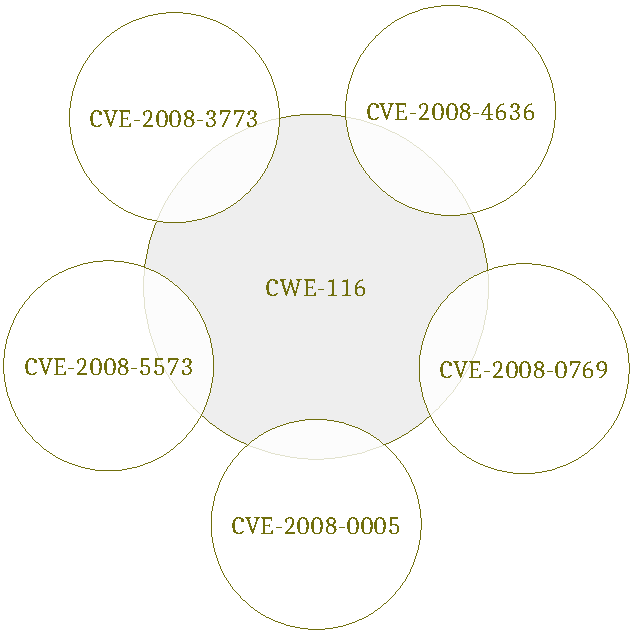
\includegraphics[width=.7\textwidth]{rcc5_CWE-116.pdf}
		\caption{Representation with RCC3}
		\label{fig:rcc5_CWE-116}
	\end{subfigure}\begin{subfigure}[b]{.5\textwidth}
		\centering
		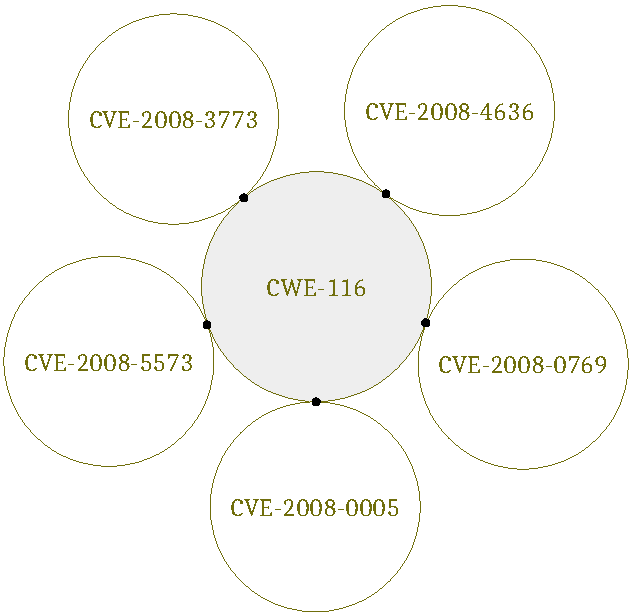
\includegraphics[width=.7\textwidth]{rcc8_CWE-116.pdf}
		\caption{Representation with RCC8}
		\label{fig:rcc8_CWE-116}
	\end{subfigure}
	\begin{subfigure}[b]{\textwidth}
		\centering
		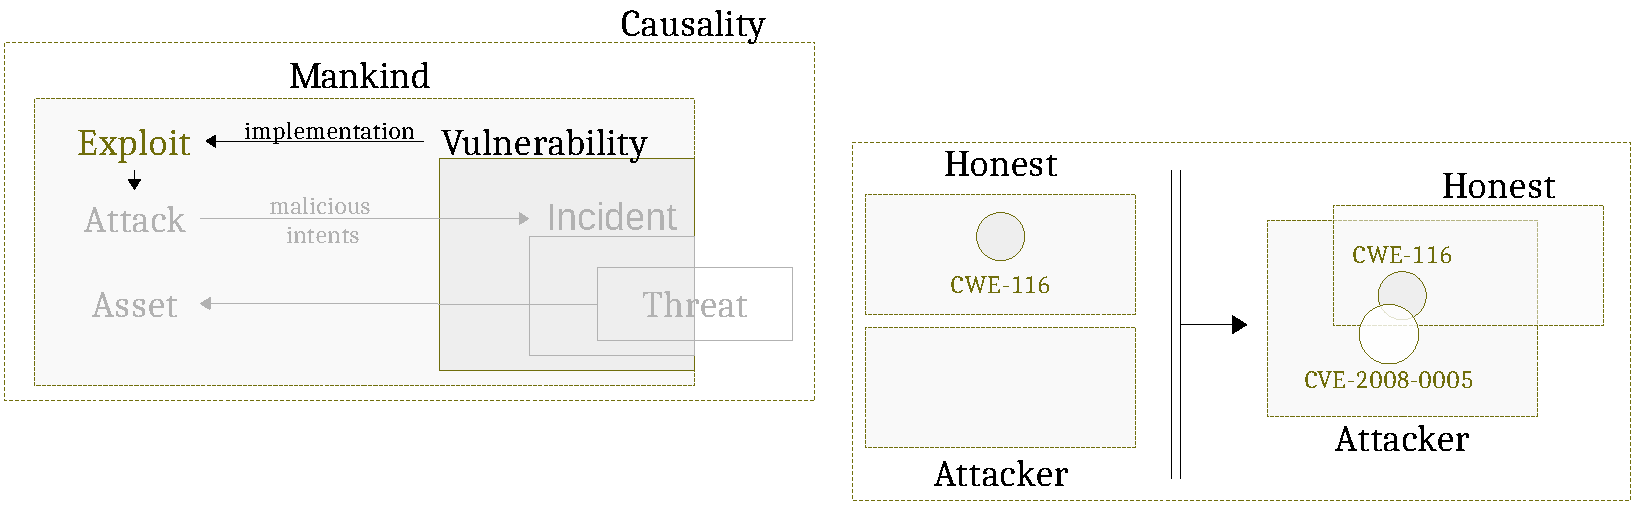
\includegraphics[width=\textwidth]{KML_CWE-116.pdf}
		\caption{Representation in K-Modal Logic}
		\label{fig:KML_CWE-116}
	\end{subfigure}
	\caption{Relations between CWE-116 and correlated CVEs}
\end{figure}
Definition~\ref{def:weakness} states that CWE-116 is a weakness iff there exists a world in
K Modal Logic, representing the system in which this weakness exists, 
such that the natural evolution of this system (i.e. formalized by the causality principle) 
make it possible to reach another state of the system (i.e. another, accessible world)
where there exist a vulnerability that can be implemented from CWE-116 (and this relation 
is not DR). The CWE website proposes the connection between CWE-116 and, for example, 
CVE-2008-5573; a vulnerability of the login sub-system 
of the Poll Pro v2.0\autocite{pollpro} system.
The formal relation between the two is given as a link (i.e. URI) between the CWE and
the CVE, the description of the relation is not defined but it is supposed to be
inferred from the descriptions of the CWE-CVE. 
We can formally represent this link as the ONE connection in RCC3, depicted in 
Figure~\ref{fig:rcc5_CWE-116}, or EC connection in RCC8 (Figure~\ref{fig:rcc8_CWE-116}).

\fixnote{mr}{shouldn't we consider the agent who introduces the weakness as dishonest? don't we say this in part 1?}
\end{example}

It is interesting to note that the CWE-CVE relation expresses the correlation
between weaknesses and vulnerabilities in the most simple form, such that we
can formalize all the relation as ONE in RCC3 or EC in RCC8.  To express a more
complex relation between the two we shall analyze the definition of CWE-116.
This is related to the Weakness-Vulnerability-Incident process (i.e. to the
details on the implementation/realization in Figure~\ref{fig:safety-security})
that we analyze in the next section, Section~\ref{sec:incidentaccident}.

\begin{definition}{\bf Region: Vulnerability and Defect --}\label{def:vulnerability-defect}
A region $\region\subseteq\agent$ of an agent $\agent\in\agentuniverse$ is
	called \emph{Vulnerability} if the agent $\agent$ is referred to as Mankind, 
	\emph{Defect} if the agent is referred to as Nature.
\end{definition}

\subsubsection{Process: Incidents and Accidents}\label{sec:incidentaccident}
In our informal definition depicted in Figure~\ref{fig:safety-security}, an
Incident is generated through a process caused by a Vulnerability (which,
in turn, is caused by a Weakness). Symmetrically, Nature has a process from Defect
to Accidents. We start by analyzing the process generated by Mankind, which is
divided into the following phases (as shown in Figure~\ref{fig:cwe-nvd-capec}):
\begin{enumerate}
	\item An agent (Mankind or Nature) defines a system, e.g. by following an engineering process for creating a new system, or for redesigning or improving an existing system (e.g. a component or a collection of components) 
	\item The dogmatic definition of a system contains a Weakness (i.e. the agent, Mankind or Nature, introduces an unintended behavior), for example as an un-intended behavior or as an architectural fallacy. The Weakness can be applied to the abstract definition of the system.
	\item The Weakness can be defined as a malicious process for a system, called Vulnerability (or Defect for Nature)
	\item The process expressed by the Vulnerability can be made operational for a specific implementation of the system (i.e. implemented by Mankind or realized by Nature) 
\end{enumerate}
Those additional details are depicted in Figure~\ref{fig:safety-security_2}, an update
of Figure~\ref{fig:safety-security}.

\begin{figure}[t]
	\centering
	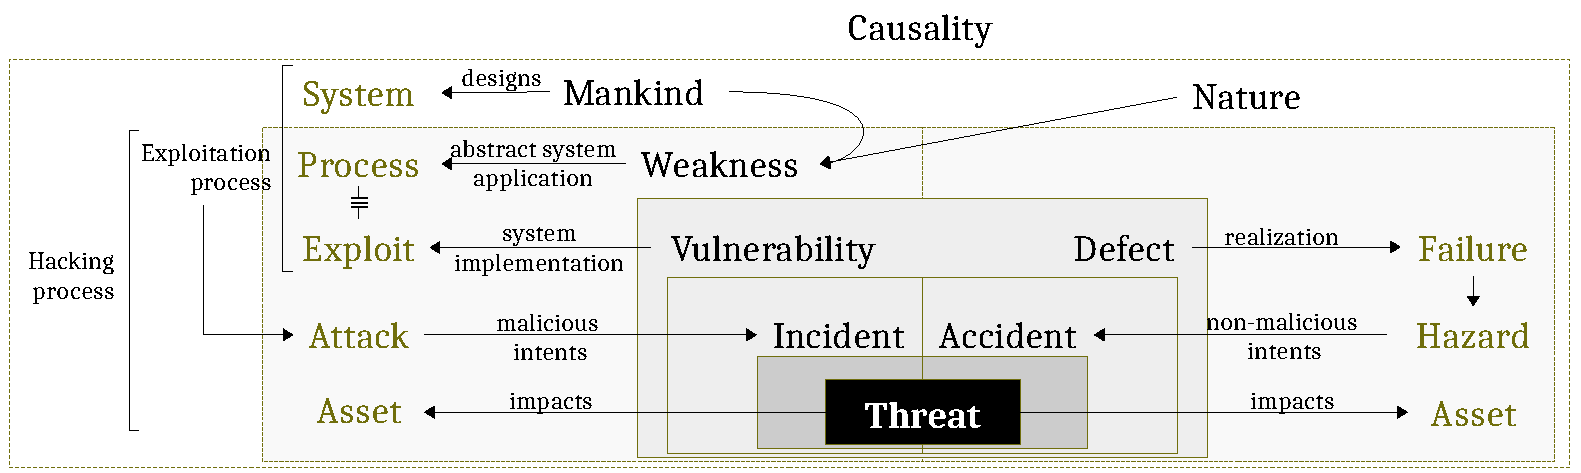
\includegraphics[width=\textwidth]{safety-security_2.pdf}
	\caption{Updated overview security and safety keywords, where Process
	has to be intended as ``Abstract Exploitation Process''}
	\label{fig:safety-security_2}
\end{figure}

\begin{definition}{\bf Exploitation Process --} An \emph{Exploit} is an \emph{implementation} of
a Vulnerability, where a Vulnerability describes how to transform a
Weakness into an abstract malicious process, which can be applied\footnote{Meaning that the
malicious process, i.e.  any structured procedure such as a protocol, can be
somehow made operational, e.g. implemented} to one or many systems. So, the act
of an agent (Mankind) of ``exploiting a Vulnerability'' is the process of
making the Vulnerability operational, by implementing the Vulnerability w.r.t.
a specific target system.  Whenever the agent is Nature, the implementation is
more broadly considered a realization\footnote{``The state of being
realized''\autocite{Merriam2020realization}}. 
\end{definition}

\begin{figure}[t]
	\centering
	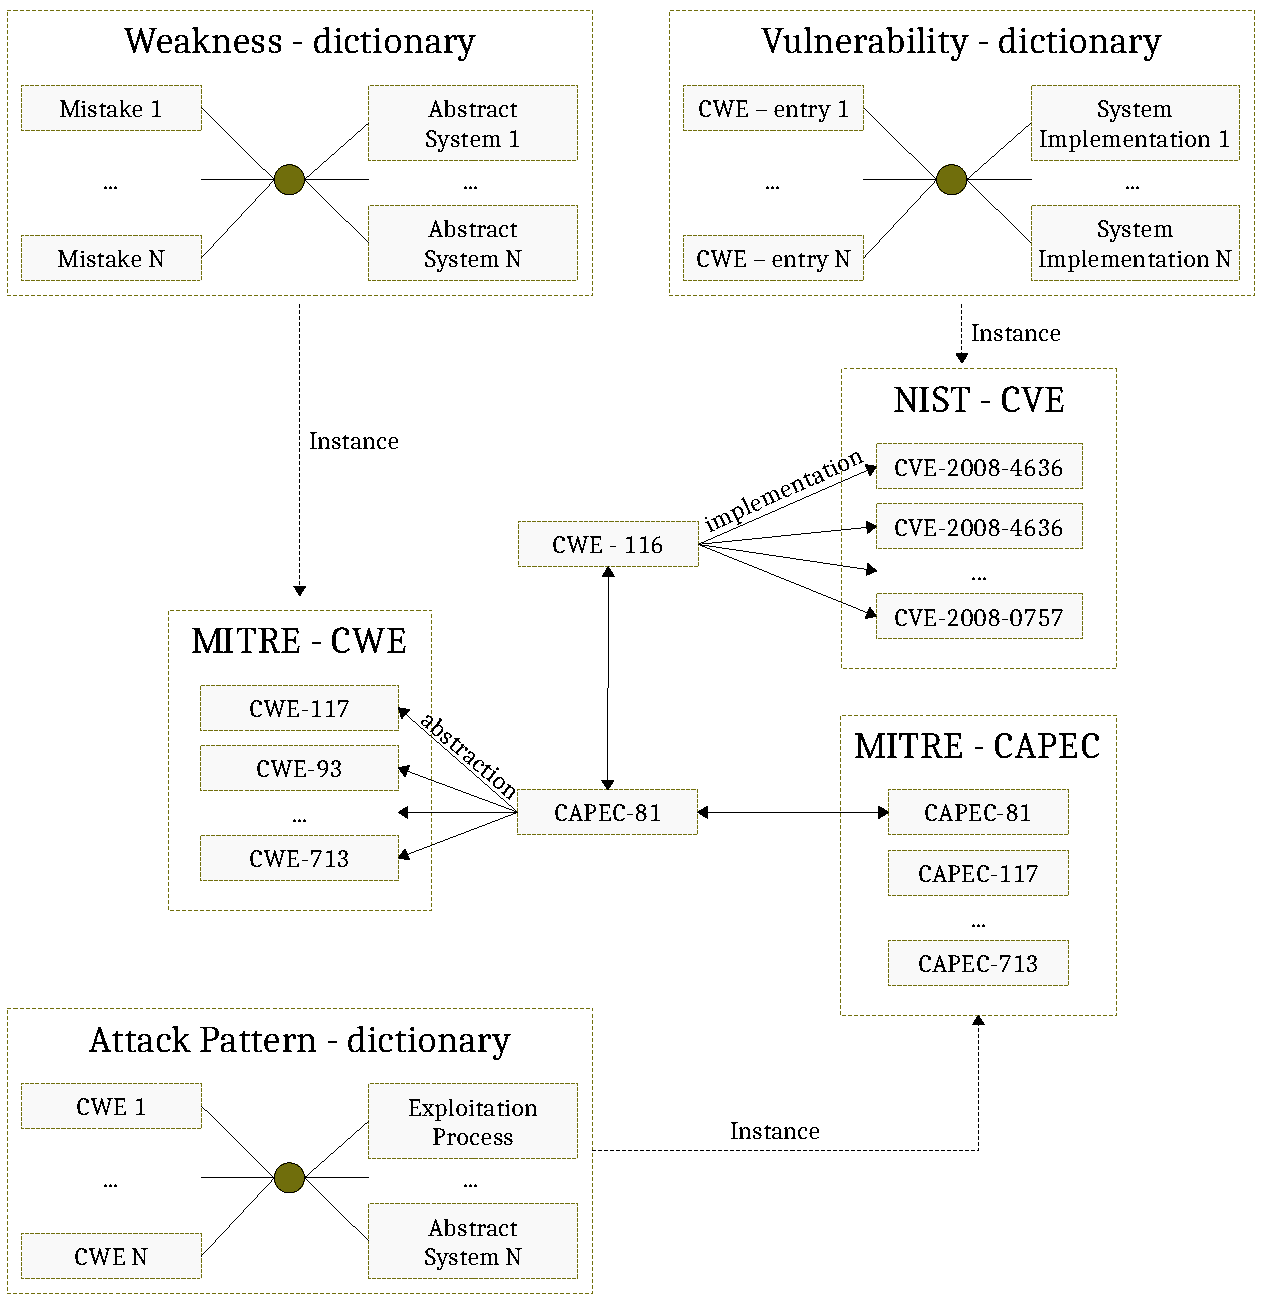
\includegraphics[width=\textwidth]{cwe-nvd-capec.pdf}
	\caption{Cybersecurity online dictionaries and connections}
	\label{fig:cwe-nvd-capec}
\end{figure}

The Common Attack Pattern Enumeration and
Classification\autocite{MITRE2020CAPEC} (CAPEC) online service provides a
``community resource'' which aims at ``identifying and understanding attacks''.
The MITRE writes on the CAPEC homepage that ``Understanding how the adversary
operates is essential to effective cyber security. CAPEC helps by providing a
comprehensive dictionary of known patterns of attack employed by adversaries to
exploit known weaknesses in cyber-enabled capabilities. It can be used by
analysts, developers, testers, and educators to advance community understanding
and enhance defenses.''. We can extrapolate two major concepts: 
\begin{itemize}
	\item While understanding the exploitation process is the aim of the
		CWE and CVE initiatives, understanding the hacking process is
		the aim of the CAPEC initiative.
	\item CAPEC provides a \emph{dictionary} of \emph{known} attack patterns.
		As stated in details in Section~\ref{sec:problem}, this dictionary contains
		empirical evidences and should not be used to induce a cybersecurity 
		theory; but it can be used to validate a theory.
\end{itemize}

\begin{example}
The CWE-116 doesn't just relate the Weakness to a number of Vulnerability in
	the CVE but also relates the Weakness to a number ($4$ for the CWE-116)
	of abstract attack path in the CAPEC:
	\begin{itemize}
		\item CAPEC-104\autocite{CAPEC-104} Cross Zone Scripting
		\item CAPEC-73\autocite{CAPEC-73} User-Controlled Filename
		\item CAPEC-81\autocite{CAPEC-81} Web Logs Tampering
		\item CAPEC-85\autocite{CAPEC-85} AJAX Fingerprinting
	\end{itemize}

	Each CAPEC entry has a reference to one or many CWE, including CWE-116.
\end{example}

After the exploitation process, as depicted in Figure~\ref{fig:cwe-nvd-capec},
another process starts and transforms a Vulnerability in an Incident by
Attacking the system with a malicious Hack, as follows.
\begin{enumerate}
\setcounter{enumi}{4}
	\item An agent (Mankind\footnote{For the sake of readability we focus
		only on Mankind as an agent}) the exploitation process can be
		used to hack a system. We use the term hack (as hacking) to
		stress that nothing prevents this process from being honest,
		however, for the sake of simplicity, we focus on Attacks which
		are malicious by definition.
	\item An Attack is applied to a system with malicious intent by an
		agent
	\item The application of the attack results in an Incident which
		impacts, i.e. poses a Threat to, an Asset
\end{enumerate}

\begin{definition}{\bf Hacking Process}\label{def:hackingprocess}
An \emph{Attack} is the act of making operational an \emph{Exploitation Process} 
	causing an Incident. 
\end{definition}

\begin{example}	CAPEC-81\autocite{CAPEC-81} Web Logs Tampering --
	\begin{itemize}
		\item Description: An attacker is able to cause a victim to
			load content into their web-browser that bypasses
			security zone controls and gain access to increased
			privileges to execute scripting code or other web
			objects such as unsigned ActiveX controls or applets.
			This is a privilege elevation attack targeted at
			zone-based web-browser security. In a zone-based model,
			pages belong to one of a set of zones corresponding to
			the level of privilege assigned to that page. Pages in
			an untrusted zone would have a lesser level of access
			to the system and/or be restricted in the types of
			executable content it was allowed to invoke. In a
			cross-zone scripting attack, a page that should be
			assigned to a less privileged zone is granted the
			privileges of a more trusted zone. This can be
			accomplished by exploiting bugs in the browser,
			exploiting incorrect configuration in the zone
			controls, through a cross-site scripting attack that
			causes the attackers' content to be treated as coming
			from a more trusted page, or by leveraging some piece
			of system functionality that is accessible from both
			the trusted and less trusted zone. This attack differs
			from "Restful Privilege Escalation" in that the latter
			correlates to the inadequate securing of RESTful access
			methods (such as HTTP DELETE) on the server, while
			cross-zone scripting attacks the concept of security
			zones as implemented by a browser. 
		\item Execution Flow: 
			\begin{enumerate}
				\item Explore: Find systems susceptible to the
					attack: Find systems that contain
					functionality that is accessed from
					both the internet zone and the local
					zone. There needs to be a way to supply
					input to that functionality from the
					internet zone and that original input
					needs to be used later on a page from a
					local zone. 
				\item Experiment: Find the insertion point for
					the payload: The attacker first needs
					to find some system functionality or
					possibly another weakness in the system
					(e.g. susceptibility to cross site
					scripting) that would provide the
					attacker with a mechanism to deliver
					the payload (i.e. the code to be
					executed) to the user. The location
					from which this code is executed in the
					user's browser needs to be within the
					local machine zone.
				\item Exploit: Craft and inject the payload:
					Develop the payload to be executed in
					the higher privileged zone in the
					user's browser. Inject the payload and
					attempt to lure the victim (if
					possible) into executing the
					functionality which unleashes the
					payload.
			\end{enumerate}
		\item Prerequisite: The target must be using a zone-aware browser. 
		\item Consequences: 
			\begin{itemize}
				\item Integrity: Modify Data
				\item Confidentiality: Read Data
				\item Confidentiality, Access Control, Authorization: Gain Privileges
				\item Confidentiality, Integrity, Availability: Execute Unauthorized Commands
			\end{itemize}
	\end{itemize}

\end{example}

The formalization of the Exploitation and Hacking processes is the
formalization of two foundational cybersecurity concepts which lay the basis
for the definition (and formalization) of the cybersecurity theory in the next
Section (Section~\ref{sec:theory}). However, the formal definition of those
processes shall (i) correlate the formal definition of agents (i.e. the
Definition~\ref{def:agent}) with the Causality principle (i.e. the
formalization of the Kripke structure in Definition~\ref{def:modallogic}), and,
most importantly, (ii) formally define a system as a structure of agents. For
the sake of clarity, we then postpone the formalization of the two processes to
the next Section.


\section{$\assertionRegion\behaviorRegion\factRegion$ -- A Security Theory}\label{sec:theory}
In order to address the problem raised by Herley, 
we shall define how to distinguish between a secure and an insecure system.
While most of the literature (and this paper so far) have
correlated the problem of in-security to the maliciousness of
agents interacting with the system, we show that security
doesn't seem to stem from a malicious nature but, rather, insecurity 
raises from the lack of well-defined security requirements for the
design process of a system. We argue that the high number
of security vulnerability reported today are simply the realization
of potential system configurations, which deviate from the nominal
behavior just because the \emph{intended behavior}\fixnote{mr}{maybe ``nominal'' instead of ``intended'' is better and behavior can be confused with the
relation between assertions and beliefs which is not what we mean} of the system is not precisely 
defined in the specification at the very early stages of the engineering process. 
A reference engineering process (so called, system security lifecycle of a product)
is described, in details, in Section~\ref{sec:process}. However,
for the sake of simplicity, the reader can assume for this section that 
we are currently dealing with just the relation between 
the specification of a system and its design.

Given that we apply our theory to \emph{systems engineering} and that
the two foundational processes (exploitation and hacking) are based on the
concept of a system, we shall begin by defining what a system is, in its
abstract form.

\subsection{A Reference Model for Cybersecurity Engineering}\label{sec:vmodel}
In order to describe the $\abf$-theory we briefly introduce the 
engineering concepts (detailed and extended in Section~\ref{sec:engineering})
underlying the $\abf$-theory; namely, the first three stages of the, so called,
engineering V-Model. Our definition is partial and we only use it for the 
sake of simplicity and to better present the theory.

The development process of a new product (a CPS in our case) 
should follow an engineering model. Our reference engineering process 
(inspired by the waterfall V-Model\autocite{waterfallvmodel}), as depicted in
Figure~\ref{fig:simplifiedvmodel}, is structured as the following ordered list
of abstraction refinement steps.
\begin{enumerate}
	\item The process starts with the definition of a \emph{specification}
		where the general requirements of the CPS are defined (e.g.
		functional, physical, network, and design).  As an example, an
		RFC of a communication or security protocol can be considered
		as the result of this first phase (e.g. see
		RFC-1\autocite{rfc1}.  In this first phase, we consider the
		architectural aspects of a CPS such as the draft physical and
		functional architectures.
	\item The process then continues with the definition of a design where
		the requirements of the previous phase holds; detailing the
		logic of the physical (e.g. the physical-layer encoding of the
		information) and functional architectures (e.g. the protocol
		logic of communication over a number of potential sessions).
	\item Finally, the design is implemented as hardware (HW) for the physical architecture
		and software (SW) for the functional architecture.
\end{enumerate}

\begin{figure}[t]
	\centering
	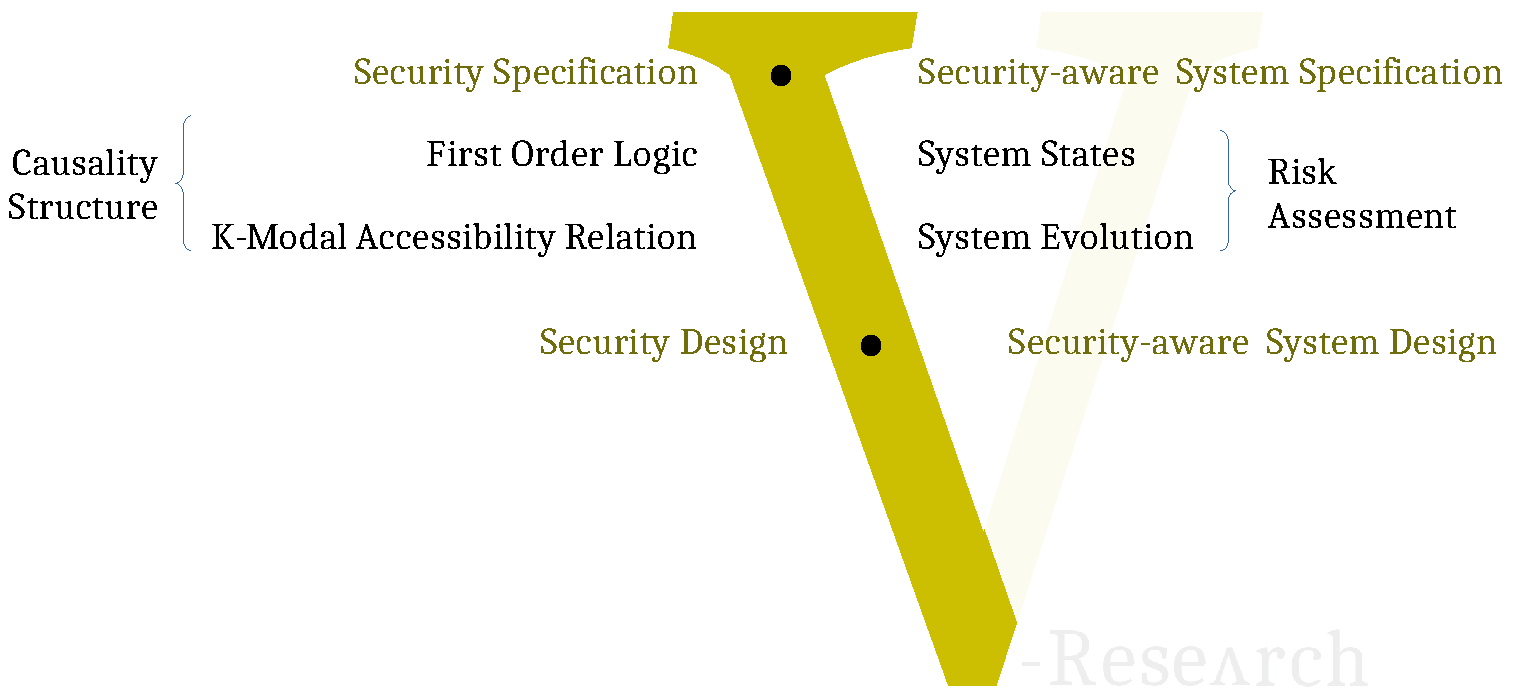
\includegraphics[width=\textwidth]{vmodel.pdf}
	\caption{Cybersecurity Engineering Life-cycle}
	\label{fig:simplifiedvmodel}
\end{figure}

\subsection{Abstract System}\label{sec:systemstate}
The ISO/IEC/IEEE 15288:2015 (System Life Cycle Processes) provides a definition
of system as ``A combination of interacting elements organized to achieve one
or more stated purposes.''\autocite{ISO201515288}.  Therefore, a system can be
considered as a single agent where its interacting elements are the
constituents of the agent itself. For the sake of simplicity we first define a
system as an agent and then extend the definition to a ``combination of
interacting'' agents.  We use the same process of \autocite{Santaca2016abf} but
over slightly different terms. The differences and commonalities with
\autocite{Santaca2016abf} are described in Appendix~\ref{app:abf}. 

There is no agreement between the research communities (e.g.
Multi-Agent-System, Epistemic Logic) on which are the constituent of an agent
as a system. However, the same ideas revolved around for thousands of years.
Some relevant examples for our objective are the following.
\begin{itemize}
	\item In \autocite{Hintikka1962knowledge}, Hintikka describes the
		difference between Knowledge and Belief (as epistemological
		concepts), and the whole Doxastic logic defines in details how
		Beliefs can be formalized.
	\item In \autocite{Hintikka1993Information}, Hintikka describes the concept
		of Information and the difference with Knowledge and Belief.
	\item In \autocite{Empiricus1990Pyrrhonism}, the author states: ``The
		logical criterion also may be used in three senses -- of the
		agent, or the instrument, or the ``according to what''; the
		agent, for instance, may be a man, the instrument either sense
		perception or intelligence, and the ``according to what'' the
		application of the impression ``according to'' which the man
		proceeds to judge by means of one of the aforesaid
		instruments.'' 
	\item In \autocite{Santaca2016abf}, the authors defines an agent as a
		tuple of Assertions, Beliefs, and Facts.
\end{itemize}

If we consider \autocite{Empiricus1990Pyrrhonism}, the author applies a
``logical criterion'' to an agent, for instance a man, for instance a device in
a system (or a system) as in \autocite{Santaca2016abf}.  The instrument identified is sense
perception, because a man is considered as example, but we can abstract from the
concept of instrument and consider any received information, where information is
considered as in \autocite{Hintikka1993Information}; which can be
summarized by the following axiom: ``Information is specified by specifying
which alternatives concerning the reality it admits and which alternatives
excludes''. This means, for our argument, that considering a propositional
variable, which admits the two alternatives True/False, its information is
defined as Believed to be True/False and not Believed to be the opposite. 
%Similarly, when reasoning on a
%mereotopological region w.r.t. the RCC (e.g. RCC3 admits two regions to be
%equal, disjoint, or overlapping) information on this region should exclude
%some of the alternatives. 
Finally, in \autocite{Empiricus1990Pyrrhonism}
the author states that the logical criterium can be judged according to a frame of reference.
For our argument, as in \autocite{Santaca2016abf}, we define this concept
as Knowledge (or Facts); where knowledge is defined, as in \autocite{Steup2020epistemology}, as
a set of proposition known by an agent, such that: (i) knowledge requires belief,
(ii) knowledge require truth, (iii) knowledge must be \emph{properly justified}.

Before detailing what ``properly justified'' means, we discuss the mentioned
relation between agent and belief and we introduce a more formal definition
of knowledge and belief. For our argument, the only objective of
Information is to exchange beliefs between agents.
Due to the definition of Information and then with its relation to the probabilistic
correlation to truth/reality, we consider
information in relation with an agent's beliefs. Similarly, we consider
beliefs to define the actual behavior of an agent or a system. On the other hand,
Knowledge drives the nominal behavior of an agent or a system. This view
is not considered in most (if not all) the approaches to protocol verification
and the Dolev-Yao theory is usually applied to a representation/abstraction
of a protocol that only considers knowledge and transfer of knowledge (i.e.
if an agent sends a message, the recipient knows that message). However,
the security of a system is tightly related to the difference between
the nominal behavior and the actual (e.g. the implemented) one.

\begin{definition}{\bf System State and State-Space --}\label{def:system}
	The state of a system (or a sub-system) $s$ is identified with an
	instance of an agent state (see Definition~\ref{def:agent}) such that
	$s=\langle\rcc(\knowledgeRegion,\beliefRegion),\rcc(\knowledgeRegion,\informationRegion),\rcc(\beliefRegion,\informationRegion)\rangle$,
	where $\knowledgeRegion,\beliefRegion,\informationRegion$ are Regions
	of Knowledge, Beliefs, and Information respectively, and $\rcc$ is a
	specific relation between the Regions it predicates on.  The
	state-space of a system is then defined by the different $\rcc$
	relations between the three pairs of Regions defining the system and
	all the sub-systems.
\end{definition}
Therefore, a system state space can be seen as a superposition of multiple agent states where knowledge,
beliefs, and information are related between each other (in a mereotopological
space) through all the admissible RCC relations. 
\fixnote{mr}{are the next lines redundant?}A \emph{system state} (as an instance of the system state space)
is a specific configuration of
the $\rcc$ relations between the three regions. Therefore, a collection of 
system states defines a collection of choices for those $\rcc$ relations.

% \item  ``normally concern the state or the history of the entire universe but only
% of some small part of
% it''.  
% \item  ``Information and probability are inversely related'', i.e. ``
% the more alternatives a proposition admits of, the more probable and the less
% informative it is, and vice versa''

\begin{figure}[t]
	\centering
	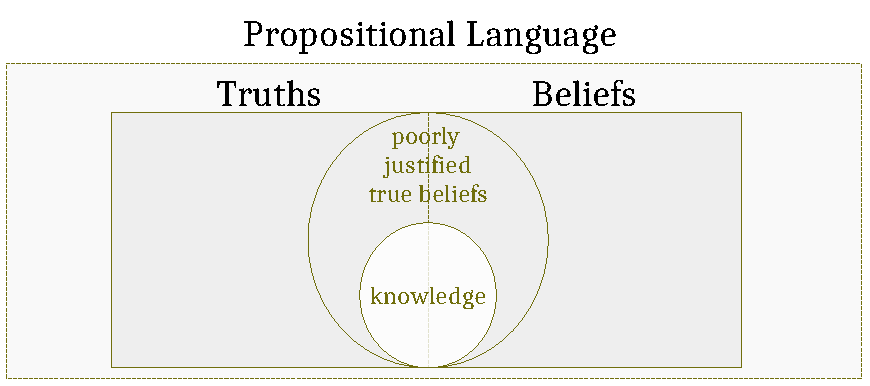
\includegraphics[width=.8\textwidth]{knowledge-belief.pdf}
	\caption{Informal representation of Knowledge and Belief}
	\label{fig:knowledge-belief}
\end{figure}

The difference between Knowledge and Belief is depicted in
Figure~\ref{fig:knowledge-belief} (see \autocite{wiki-knowledgebelief}).  However,
according to\autocite{Gettier2012knowledge},
Knowledge\footnote{``\emph{Theaetetus}: [\ldots] He said that knowledge was
true opinion accompanied by reason, but that unreasoning true opinion was
outside of the sphere of knowledge; and matters of which there is not a
rational explanation are unknowable -- yes, that is what he called them -- and
those of which there is are knowable. [\ldots] \emph{Socrates}: [\ldots] the
primary elements of which we and all else are composed admit of no rational
explanation; for each alone by itself can only be named, and no qualification
can be added, neither that it is nor that it is not, for that would at once be
adding to it existence or non-existence, whereas we must add nothing to it, if
we are to speak of that itself alone.  [\ldots]'' Plato -- Theaetetus 201
\autocite{Plato1914Plato}} as an epistemological concept is difficult to formally define. 
Similarly for the concept of information, Hintikka in \autocite{Hintikka1993Information}
states that ``A purely logical definition of information is impossible''.
In this work, however, we are not interested in how knowledge, information, or
belief can be precisely formalized from an epistemic standpoint.  We assume
that a semantic of a correct (i.e. commonly believed to be true) definition of epistemic knowledge exists, for
example the one given in\autocite{Hintikka1962knowledge} by Hintikka, and we
then define knowledge in terms of the Kripke structure defined in
Definition~\ref{def:modallogic}; similarly for Belief.

\begin{definition}{\bf Knowledge --}\label{def:knowledge}
Given an abstract collection of Agents $Ag$, and the modal operator
	$\knows{a}{}$ (where $a\in Ag$), Knowledge is defined as a region 
	of predicates known by an agent $\knowledge{a}=\bigcup_\Phi \knows{a}{\varphi}$ 
	(where $\Phi$ is the collection of all the propositions known by $a$).
	Given a proposition $P$, we extend the semantics of the Causality structure with:
	\begin{enumerate}[noitemsep]
		\item[$(\interpretation16)$] $\world\models\knows{a}{P}$ iff
			$\world'\models P$ for all $\world'$ such that
			$\world\modalrelation\world'$.
	\end{enumerate}
\end{definition}

\begin{definition}{\bf Belief --}\label{def:belief}
	Given an abstract collection of Agents $Ag$, and the modal operator
	$\believe{a}{}$ (where $a\in Ag$), Belief is defined as a region 
	of predicates believed by an agent $\belief{a}=\bigcup_\Phi \believe{a}{\varphi}$
	(where $\Phi$ is the collection of all the propositions believed by $a$).
	Given a proposition $P$, we extend the semantics of the Causality structure with:
	\begin{enumerate}[noitemsep]
		\item[$(\interpretation17)$] $\world\models\believe{a}{P}$ iff
			$\world\models\neg\knows{a}{\neg P}$ (i.e. the agent $a$ considers $P$ possible) 
			and $\world'\models P$ for all
			$\world'$ such that $\world\modalrelation\world'$.
	\end{enumerate}
\end{definition}

\begin{definition}{\bf Information --}\label{def:information}
	Given an abstract collection of Agents $Ag$, and the modal operator
	$\informs{a}{}$ (where $a\in Ag$), Information is defined as a region 
	of beliefs asserted by an agents $a$.
	%and transferred from $a$ to $b$ ($a\rightarrow b$).
	$\information{a}=\bigcup_\Phi \informs{a}{}{\varphi}$
	(where $\Phi$ is the region of all the propositions believed and asserted by $a$).
	Given a proposition $P$, we extend the semantics of the Causality structure with:
	\begin{enumerate}[noitemsep]
		\item[$(\interpretation18)$] $\world\models\informs{a}{P}$ iff
			$\world\models\belief{a}{P}$ (i.e. the agent $a$ considers $P$ possible), 
			$\world\models\neg\belief{a}{\neg P}$%, 
			%and $\world'\models P$ for all
			%$\world'$ such that $\world\modalrelation\world'$.
	\end{enumerate}
\end{definition}

\subsection{Operational System}\label{sec:engsystemstate}
When dealing with a specification of a system (i.e. the design if the system
for a specific operation (as a generic operating/operational system),
considering abstract and general concepts such as knowledge, belief, or
information may result to be too abstract for the objectives of the overall engineering
process (e.g. verification and validation).
As an example, we are usually not
interested in information in abstract but to the transfer of that
information, which we call Assertions, made by a subset of agents. 
Therefore, we now define how we consider an agent for the engineering
of CPS.

\begin{enumerate}
	\item We consider Information only when the intention of exchanging 
		that Information is from a sender to 
		recipient is defined; and we call it \emph{Assertion}  
	\item Similarly, the portion of Beliefs we consider for system
		engineering is the one that builds (input) or describes
		(output) the behavior of an agent (strategy rules
		\footnote{``The logical structure of information is one of the
		most basic and one of the most basic and one of the simplest
		thing in the wide and wonderful world of logical analysis. This
		point can be put in a deeper perspective. A distinction
		[\ldots] ought to be made [--] between two kinds of rules (or
		principles) in any strategic activity like knowledge seeking.
		On the one hand you have the rules that define the game, e.g.
		how chessmen are moved on a board. The can be called
		\emph{definitory} rules.  They must be distinguished from rules
		[\ldots] that deal with what is better and what is worse in the
		game in question.  Definitory rules do not say anything about
		this subject. Rules which do can be called \emph{strategic
		rules}'' -- Hintikka in \autocite{Hintikka1993Information}}),
		and
	\item We consider a set of axiomatic \emph{Facts} (definitory rules) instead
		of considering the more general epistemic definition of
		Knowledge. Specifically, Facts describes:
		\begin{itemize}
			\item The functional architecture of each agents
			\item The physical/structural (HW/SW) architecture of each
				subsystem of agents and agent within a
				subsystem
			\item Other important aspects of the system that we
				describe afterwards in this paper, such as
				the assets and security properties 
		\end{itemize}
\end{enumerate}
We give a graphical representation of (sub-)system and agent in Figure~\ref{fig:system-agent}.

We note here (and describe with more details afterwards in this paper) that the
data flow can be defined as a transfer of Beliefs through Assertions (i.e. the
Beliefs flow).

\begin{figure}[t]
	\centering
	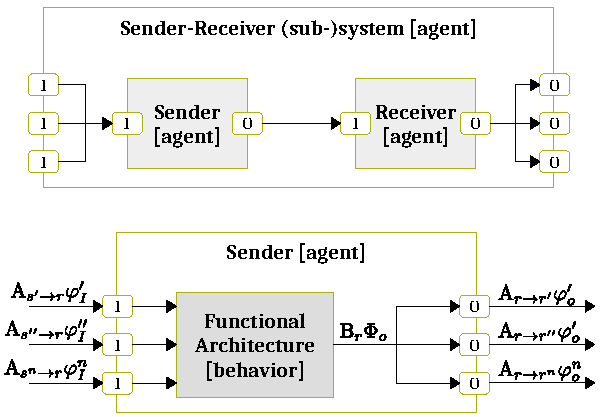
\includegraphics[width=.9\textwidth]{system-agent.pdf}
	\caption{Example of system and agent structure}
	\label{fig:system-agent}
\end{figure}

\begin{definition}{\bf Assertion -- }\label{def:assertion}
	An assertion (\fix{mr}{subtype of Information}) of  is an intended transfer of beliefs between
	two agents $a$ and $b$ such that
	\begin{enumerate}[noitemsep]
		\item[$(\interpretation19)$] $\world\models\rassert{a}{b}{P}$ iff
			$\world\models\belief{a}{P}$, 
			$\world\models\neg\belief{a}{\neg P}$, 
			$\world'\models\rcc(\belief{a}{P},\belief{b}{P})$, 
			for all $\world'$ such that $\world\modalrelation\world'$.
	\end{enumerate}
\end{definition}

\begin{definition}{\bf Behavior -- }\label{def:behavior}
	The behavior (\fix{mr}{subtype of Beliefs}) of an agent is defined as the transformation process (e.g. defined as a
	protocol, or a functional architecture) that determines the
	output-beliefs based on input-beliefs and vice versa (where input-beliefs and
	output-beliefs are beliefs taken as input or output respectively).
	\begin{enumerate}[noitemsep]
		\item[$(\interpretation20)$] $\world\models\bigcup_{\Phi}\believe{s}{\varphi}$ and $\world\models\behave{a}{[\bigcup_{s\in S}\believe{s}{P_{s}}]}$ iff
			$\world\models\belief{a}{P'}$, 
			
		where $a$ is an agent, $S$ is a set of agents such that $a\neg\in S$, and the calculation of $P'$ is deteministic.
	\end{enumerate}
\end{definition}

\begin{definition}{\bf Fact -- }\label{def:fact}
	Facts are a \fix{mr}{sub-region/subtype} of Knowledge $\factRegion = \bigcup_\Phi \knows{a}{\varphi}$
	that predicate in a factive way, e.g.
	if $a$ knows that $P$ then $P$, and the region of facts is monotone (no revision).
	\begin{enumerate}[noitemsep]
		\item[$(\interpretation21)$] $\world\models\fact{a}{P}$ iff
			$\world \models \Box P$. 
	\end{enumerate}
\end{definition}

\begin{definition}{\bf Operational System State --}\label{def:system}
	An operational system (or a sub-system) is represented as an agent (see Definition~\ref{def:agent}) and then defined by the resulting state space,
	such that
	$s=\langle\rcc(\factRegion,\behaviorRegion),\rcc(\factRegion,\assertionRegion),\rcc(\behaviorRegion,\assertionRegion)\rangle$,
	where $\assertionRegion,\behaviorRegion,\factRegion$, are regions of assertions, behavior (i.e. the beliefs generated by the behavior), and facts respectively.
\end{definition}

As already presented in \autocite{Santaca2016abf} it follows that, defining
a system (or an operational system) with a fixed number of regions, there exist
an upper-bound to the number of possible configuration of a system, defined by
the possible relations between the different regions.
For completeness, we report in the next paragraph 
the calculation done in \autocite{Santaca2016abf}.

\Paragraph{Number of different configurations of a system}
The general formula to calculate the number of different types of agents is
$r^{\binom{n}{k}}$, where $r$ is the number of relations with arity $k$,
between $n$ different sets, where $r^e$ is the number of permutation of $r$
relations over $e$ elements with repetitions, with $e$ being the number of
$k$-ary combinations of $n$ sets, $\binom{n}{k}$.
In our case, $\binom{n}{k}=3$ since we consider $3$ sets
($\assertionRegion,\behaviorRegion,\factRegion$), and all the relations
considered in the RCC are binary.  Hence, using RCC5 (with five different
spatial relations) over three sets, we can theoretically define up to 125
different type of agents. However, only 54 of the 125 (as showed in
\cite{improvingRCC}) combinations are topologically correct with respect to
the definition of the relations of RCC5. Generalizing to all the RCCs:

\begin{itemize}%[nosep]
\item \emph{RCC3} --- theoretical: $3^3=27$,  correct: 15 
\item \emph{RCC5} --- theoretical: $5^3=125$, correct: 54
\item \emph{RCC8} --- theoretical: $8^3=512$, correct: 193
\end{itemize}

Hence, even if considering a different number of sets than the three
$\assertionRegion$, $\behaviorRegion$ and $\factRegion$ exponentially affects
the number of theoretical agents, the application of RCC downscales that number
of a factor that ranges from 1.8 to 2.5. In addition, using RCC5 we consider
3.6 times more (different) types of agents than RCC3, but using RCC8 would
allow us to consider 3.5 times more different agents.

In the quantitative evaluation of a single agent, depicted in Figure~\ref{fig:quantitative},
we argue that only 1 configuration represents the nominal (expected) behavior 
of the agent while the other configurations are either impossible to 
implement or diverge from the intended nominal behavior. We note 
that, the numbers reported here do not consider the details of the
engineering process and should be considered a limit of an abstract 
representation of the system. In Section~\ref{sec:engineering} we
detail this numeric evaluation to faitfully represent the
number of insecurity configurations.

\begin{figure}[t]
	\centering
	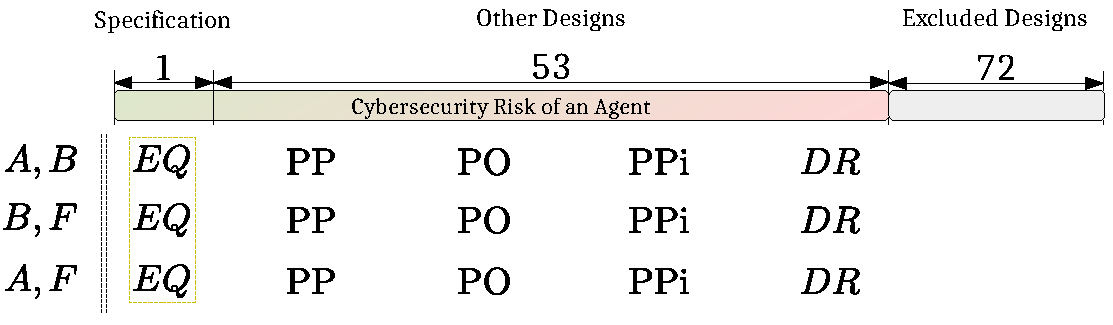
\includegraphics[width=.9\textwidth]{quantitative.pdf}
	\caption{Quantitative representation of the cybersecurity risk for a single agent}
	\label{fig:quantitative}
\end{figure}

As described beforehand in this section, the collection of Facts shall define
the functional and the physical architecture of an agent, but Assets and
security properties are defined as Facts, i.e. true. Given that understanding
why an Asset is considered as such by the user doesn't necessarily allow
us to better qualify an Asset, we consider the fact of ``being an asset'' as
a predicate \fix{mr}{(or a true function)} of a component of a system. 

\begin{definition}{\bf Asset --}\label{def:asset}
For any agent $a\in Ag$ in a collection of Agents $Ag$, an agent is considered an asset iff 
	\begin{enumerate}[noitemsep]
		\item[$(\interpretation22)$] $\world\models\asset{a}$ iff
			$\world\models \Box\asset{a}$.
	\end{enumerate}
\end{definition}

The definition of the security properties is given in Section~\ref{sec:properties}

\subsection{Qualitative Evaluation of Agent Space in $\abf$}\label{sec:agentspace}
While a quantitative analysis reveals how many possible configurations of an
agent (i.e. a system) exist w.r.t. the $\abf$ theory (i.e. $54/125$ in RCC5), a
qualitative analysis of the different configurations describes
the configurations allowed by the $\abf$ theory, and how those configurations can be
categorized.  In Table~\ref{tab:5com} we provide the generic composition table
of RCC5 over 3 regions instantiated over $\abf$, which shows the whole state
space for a single agent. The color coding of the table represents the 
risk function as a risk matrix as we detail afterwards in this section.

A detailed qualitative categorization of agents over a theory similar to the
$\abf$ one, is presented in this article and described in
\autocite{Santaca2016abf}. The differences in the formalization and of the
application requires another in-depth analysis. As depicted in
Figure~\ref{fig:soundness}, the relation between Facts, and Assertions and Behavior
defines the soundness of the design (admissible configurations of Assertions,
Behaviors and, in turn, Beliefs) w.r.t. the specification (what the
specification mandates, such as by the nature of the physical/functional
architectural models). We categorize agents by first analyzing the relations
between each pair of Regions defining an agent (i.e. $\abf$), and then we
categorize the different agents as tuple of the three Regions.
For the sake of simplicity, soundness is opposed to non-soundness in the following, however,
with the RCC we consider different ``degrees'' of soundness. For example,
in RCC5, if we consider EQ between two Regions as representing soundness, DR over the same Regions
represents non-soundness while PP, PO, PPi represents the different degrees of soundness.

\begin{figure}[t]
	\centering
	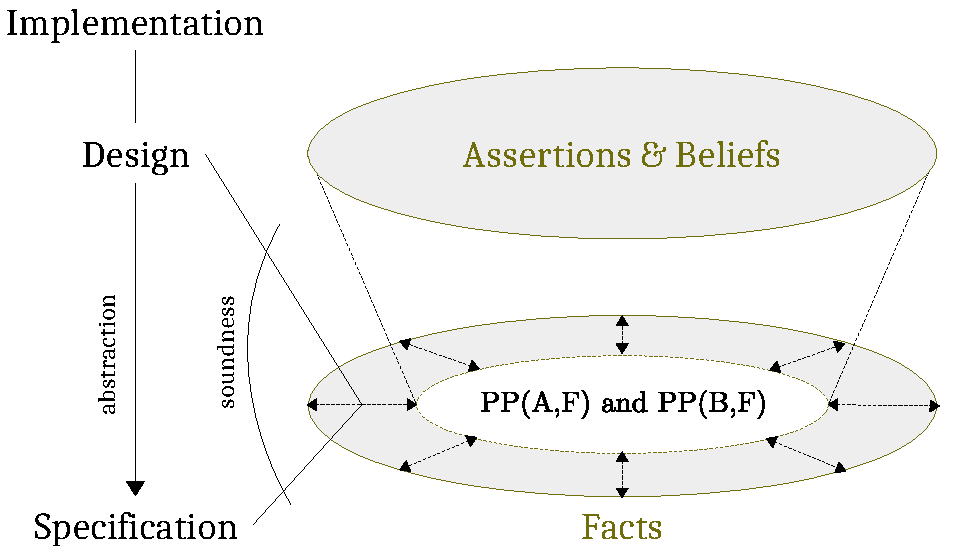
\includegraphics[width=.8\textwidth]{soundness.pdf}
	\caption{Example relation between Facts, and Assertions and Beliefs}
	\label{fig:soundness}
\end{figure}

\Paragraph{\Rcc{$\assertionRegion$}{$\behaviorRegion$} -- Collaboration}
In order to reason on the relation between assertions and behavior we first
need to consider that, by definition, assertions are defined as transfer of
information between two agents, e.g., $a$ and $b$.  Therefore, as depicted in
Figure~\ref{fig:system-agent}, an agent has two main categories of assertions,
input and output assertions.  Given an agent $a$ and a collection of asserted
predicates $\Phi$, the Input assertions are those received by $a$ from an agent
$s$ acting as a sender, $\rassert{s}{a}{\Phi}$; similarly, output assertions
are sent from $a$ to a receiver $r$, $\rassert{a}{r}{\Phi}$. We shall consider
two pairs of regions\footnote{``I am not asserting, as Lotze did, that a relation between $X$ and $Y$
consists of a quality in $X$ and a quality in $Y$ -- a view which I regard as
quite indefensible. -- I assert that a relation $Z$ between $X$ and $Y$ involves
the existence in $X$ of the quality ``having the relation $Z$ to $Y$'' so that
a difference of relations always involves a difference in quality, and a
change of relations always involves a change of quality.'' --  Ellis J. McTaggart, The Unreality of Time\autocite{Mctaggart1908unreality}}: 
\begin{itemize}
	\item \Rcc{$\assertionRegion_{s\rightarrow a}$}{$\behaviorRegion$},
		where the relation between Input-assertions and behavior
		describes the soundness of the execution of the functional
		architecture w.r.t. input elicitation. With more details, the
		ideal specification of the functional architecture, along with
		the expected inputs, defines the functional behavior of an
		ideal system.  If all the inputs (Assertions) are correctly
		handled in the functional specification (behavior) the
		specification is sound. 

	\item \Rcc{$\assertionRegion_{a\rightarrow r}$}{$\behaviorRegion$},
		where the relation between behavior and outputs describes the
		completeness of the behavior defined in the specification
		w.r.t. the input elicitation.  With more details, if all the
		outputs (assertions) of the functional architecture can be
		produced, the functional architecture is complete.
\end{itemize}


\Paragraph{\Rcc{$\assertionRegion$}{$\factRegion$} and \Rcc{$\behaviorRegion$}{$\factRegion$} -- Honesty and Competence}
While Assertions and Beliefs generated by the Behavior determines how a system should work, and the
relation between the two defines the quality (i.e. the completeness w.r.t the specification) of the agent, the relation of
Assertions and Behavior with Facts determines the quality with respect to the
nominal (specified) system.  Given that Facts defines what is true in the
system (e.g. the level of water in a tank may be considered as a Fact, while
the reading of a sensor as a Belief), the relation of Assertions an Facts
determines the degree of quality between the information circulating in a
system (or within an agent) and reality.  Since the transfer of information through Assertions
generates Beliefs, a dishonest agent may circulate false information,
generating false Beliefs.  We note that it is often implied that the intention behind
circulating false information discerns a dishonest and an incompetent agent,
however, we consider honesty related to truth rather than related to what is
true\footnote{``[\ldots] truth exists only in the good man, but the true in the bad
man as well; for it is possible for the bad man to utter something true.''
Sextus Empiricus, Outlines of Pyrrhonism, II-83\autocite{Empiricus1990Pyrrhonism}}.  This implies that the
relation between Beliefs and Facts determines the competence (on the subjected
defined by the Facts) of an agent (i.e. the more competent an agent is, the
more likely a Belief of that agent is true).



\subsubsection{$\abf$ Security Enumeration (SE)} The following security requirement for a CPS specification can be summarized:
\begin{enumerate}
	\item[SE-$1$] Proper interaction between multiple correctly-behaving agents (in
		contrast with the ``Improper Interaction Between Multiple
		Correctly-Behaving Entities'' defined by the CWE--$435$ as one of the top ``view'' of the ``research concepts'' in
		\autocite{MITRE2020CWEresearch}) is defined as $\eq{\assertionRegion_a}{\behaviorRegion_a}$ for an agent $a$
	\begin{enumerate}
		\item[SE-$1.1$] The equality relation $\eq{\assertionRegion_{s\rightarrow a}}{\behaviorRegion_a}$
			describes the intended secure behavior as: the beliefs generated by the behavior of the functional architecture
			shall be complete w.r.t. the specified inputs of the agent. Therefore, \emph{the assertions received by an agent or a system
			shall be compliant with the expected inputs of the functional architecture}. For example, the inputs
			of the user of a SW must be sanitized to exclude deviations w.r.t. the expected inputs of the functions
			implemented in the SW. Another example is the type checking between allowed inputs and expected inputs.
		\item[SE-$1.2$] Similarly, the equality relation $\eq{\assertionRegion_{a\rightarrow r}}{\behaviorRegion_a}$ defines that
			the outputs of an agent $a$ shall be the outputs of the functional architecture.
	\end{enumerate}
	\item[SE-$2$]Sufficient Control Flow Management (in contrast with
		the ``Insufficient Control Flow Management'' defined by MITRE
		in the CWE--$691$ as one of the top ``view'' of the ``research
		concepts'' in\autocite{MITRE2020CWEresearch}) is defined as
		$\eq{\assertionRegion}{\factRegion}$.
	\item[SE-$3$] Correct Calculation (in contrast with the ``Improper
		Calculation'' defined by MITRE in the CWE--$682$ as one of the
		top ``view'' of the ``research concepts''
		in\autocite{MITRE2020CWEresearch}) is defined as
		$\eq{\beliefRegion}{\factRegion}$.
\end{enumerate}

We are now in the position to define what a secure system (with respect to the $\abf$-theory) is
and, based on that definition, what the security risk is and how to quantify it in a risk matrix.
\begin{definition}{\bf Security of a System or an Agent --}\label{def:security}
	A secure system is a system where SE-$1$, SE-$2$, and SE-$3$ holds for each 
	agent composing the system.
\end{definition}
The ISO 31000 consider risk as the ``effect of uncertainty on objectives'' and the refers
both of positive and negative consequences of uncertainty. Accordingly, we consider
risk as follows. 
\begin{definition}{\bf Risk --}
The whole space of potential designs of a specification with respect to the
$\abf$-theory.
\end{definition}
The definition of Risk leads to the risk matrix in Figure~\autoref{fig:quantitative}, defined as follows.
\begin{definition}{\bf Risk Matrix --}
	The risk matrix is a function between the three relations 
	$s=\langle\rcc(\factRegion,\behaviorRegion),\rcc(\factRegion,\assertionRegion),\rcc(\behaviorRegion,\assertionRegion)\rangle$,
	where the maximum risk is defined by the $DR$ relation between the three groups of Regions, and the 
	minimum risk by the $EQ$ relation over the same Regions. In between the two extremes, the granularity
	of possible intermediate configuration is defined by the calculus used (RCC5 in our case).
\end{definition}
We note that often the risk matrix is defined by the relation between likelihood and impact.
We argue that the likelihood is related to the number of possible non secure (i.e. non maximum secure) 
configurations of a system and, similarly, the impact.

\begin{table}[t]
\centering
\begin{adjustbox}{width=\textwidth}
\begin{tabular}{r||c|c|c|c|c} 
& \dr{$\assertionRegion$}{$\behaviorRegion$} & 
	\po{$\assertionRegion$}{$\behaviorRegion$}& 
	\pp{$\assertionRegion$}{$\behaviorRegion$} &
	\ppi{$\assertionRegion$}{$\behaviorRegion$} & 
	\eq{$\assertionRegion$}{$\behaviorRegion$} \\
\hline
\hline %dr
 \multirow{3}{*}{\dr{$\behaviorRegion$}{$\factRegion$}} & 
	\cellcolor{abfred} & %dr
	\cellcolor{abf-rg-1}\dr{$\assertionRegion$}{$\factRegion$} & %po
	\cellcolor{abf-rg-2}\multirow{3}{*}{\dr{$\assertionRegion$}{$\factRegion$}} & %pp
	\cellcolor{abf-rg-3} \dr{$\assertionRegion$}{$\factRegion$}& % ppi
	 \cellcolor{abf-rg-4} \\ % eq
& \cellcolor{abfred}\all{$\assertionRegion$}{$\factRegion$}& %dr
	\cellcolor{abf-rg-1}\po{$\assertionRegion$}{$\factRegion$} & %po
	\cellcolor{abf-rg-2}\dr{$\assertionRegion$}{$\factRegion$} & %pp
	\cellcolor{abf-rg-3}\po{$\assertionRegion$}{$\factRegion$} & %ppi
	\cellcolor{abf-rg-4}\dr{$\assertionRegion$}{$\factRegion$}\\ % e q
 & \cellcolor{abfred}& %dr
	\cellcolor{abf-rg-1}\pp{$\assertionRegion$}{$\factRegion$} & %po
	\cellcolor{abf-rg-2}  & %pp
	\cellcolor{abf-rg-3}\pp{$\assertionRegion$}{$\factRegion$} & %ppi
	\cellcolor{abf-rg-4} \\ %eq
\hline %po
 \multirow{3}{*}{\po{$\behaviorRegion$}{$\factRegion$}} &
	\cellcolor{abf-rg-1}\dr{$\assertionRegion$}{$\factRegion$} & %dr
	\cellcolor{abf-rg-2} & %po
	\cellcolor{abf-rg-3}\dr{$\assertionRegion$}{$\factRegion$} & %pp
	\cellcolor{abf-rg-4}\po{$\assertionRegion$}{$\factRegion$} & %ppi
	\cellcolor{abf-rg-5} \\ %eq
 & \cellcolor{abf-rg-1}\po{$\assertionRegion$}{$\factRegion$} & %dr
	\cellcolor{abf-rg-2} \all{$\assertionRegion$}{$\factRegion$} & %po 
	\cellcolor{abf-rg-3}\po{$\assertionRegion$}{$\factRegion$} & %pp
	\cellcolor{abf-rg-4}\ppi{$\assertionRegion$}{$\factRegion$} & %ppi
	\cellcolor{abf-rg-5} \po{$\assertionRegion$}{$\factRegion$}\\%eq
 & \cellcolor{abf-rg-1}\pp{$\assertionRegion$}{$\factRegion$} & %dr
	\cellcolor{abf-rg-2} &  %po
	\cellcolor{abf-rg-3}\pp{$\assertionRegion$}{$\factRegion$} & %pp
	\cellcolor{abf-rg-4}& %ppi
	\cellcolor{abf-rg-5}\\ %eq
\hline %pp
 \multirow{4}{*}{\pp{$\behaviorRegion$}{$\factRegion$}} &
	\cellcolor{abf-rg-2}\dr{$\assertionRegion$}{$\factRegion$} & 
	\cellcolor{abf-rg-3}&
	\cellcolor{abf-rg-4} & %pp
	\cellcolor{abf-rg-5}\po{$\assertionRegion$}{$\factRegion$} & %ppi
	\cellcolor{abf-rg-6}\\ %eq
 & \cellcolor{abf-rg-2}\po{$\assertionRegion$}{$\factRegion$} & 
	\cellcolor{abf-rg-3}\po{$\assertionRegion$}{$\factRegion$} & 
	\cellcolor{abf-rg-4}\pp{$\assertionRegion$}{$\factRegion$} & %pp
	\cellcolor{abf-rg-5}\eq{$\assertionRegion$}{$\factRegion$} & %ppi
	\cellcolor{abf-rg-6}\pp{$\assertionRegion$}{$\factRegion$} \\ %eq
 & \cellcolor{abf-rg-2}\pp{$\assertionRegion$}{$\factRegion$} & 
	\cellcolor{abf-rg-3}\pp{$\assertionRegion$}{$\factRegion$} & 
	\cellcolor{abf-rg-4} & %pp
	\cellcolor{abf-rg-5}\pp{$\assertionRegion$}{$\factRegion$} & %ppi
	\cellcolor{abf-rg-6} \\ %eq
 & \cellcolor{abf-rg-2}&
 	\cellcolor{abf-rg-3} & 
	\cellcolor{abf-rg-4}& %pp
	\cellcolor{abf-rg-5}\ppi{$\assertionRegion$}{$\factRegion$} & %ppi
	\cellcolor{abf-rg-6} \\ %eq
\hline %ppi
 \multirow{3}{*}{\ppi{$\behaviorRegion$}{$\factRegion$}} &
 	\cellcolor{abf-rg-3}\multirow{3}{*}{} &
 	\cellcolor{abf-rg-4}\dr{$\assertionRegion$}{$\factRegion$} &
 	\cellcolor{abf-rg-5}& %pp
 	\cellcolor{abf-rg-6}& %ppi
 	\cellcolor{abf-rg-7} \\ %eq
& \cellcolor{abf-rg-3}\dr{$\assertionRegion$}{$\factRegion$} &
 	\cellcolor{abf-rg-4}\po{$\assertionRegion$}{$\factRegion$} & 
 	\cellcolor{abf-rg-5}\all{$\assertionRegion$}{$\factRegion$}& %pp
 	\cellcolor{abf-rg-6}\ppi{$\assertionRegion$}{$\factRegion$}& %ppi
 	\cellcolor{abf-rg-7}\ppi{$\assertionRegion$}{$\factRegion$}\\ %eq
& \cellcolor{abf-rg-3} & 
	\cellcolor{abf-rg-4}\ppi{$\assertionRegion$}{$\factRegion$} & 
	\cellcolor{abf-rg-5} & %pp
	\cellcolor{abf-rg-6}& %ppi
	\cellcolor{abf-rg-7}\\ %eq
\hline %eq
	\eq{$\assertionRegion$}{$\factRegion$} & 
	\cellcolor{abf-rg-4}\dr{$\assertionRegion$}{$\factRegion$} & 
	\cellcolor{abf-rg-5} \po{$\assertionRegion$}{$\factRegion$} & 
	\cellcolor{abf-rg-6}\pp{$\assertionRegion$}{$\factRegion$} & %pp
	\cellcolor{abf-rg-7} \ppi{$\assertionRegion$}{$\factRegion$} & %ppi 
	\cellcolor{abfgreen} \eq{$\assertionRegion$}{$\factRegion$}  %eq
\end{tabular}
\end{adjustbox}
\caption{RCC5 composition table over 3 regions. The results show that there
exist 54 possible relations and the coloring anticipates the ideal risk matrix
(green the secure state with low risk, red the high risk state, and a gradient
of medium risk states). 
\all{$\assertionRegion$}{$\factRegion$} = \{\dr{$\assertionRegion$}{$\factRegion$}, \po{$\assertionRegion$}{$\factRegion$}, \pp{$\assertionRegion$}{$\factRegion$}, \ppi{$\assertionRegion$}{$\factRegion$}, \eq{$\assertionRegion$}{$\factRegion$}\}
\label{tab:5com}}
\end{table}

\subsection{System Security Evolution}\label{sec:systemevoution}
\fix{mr}{
Facts should be correlated to the causality principle. Therefore a
specification in opnet should be translated into vmt and by bounded model
checking with nuxmv identify a path towards an undesired state, if that fails
use abf to mutate the first state into one of the possible according to abf and
re-run nuxmv.

Knowledge is the theory itself, an instance is the facts of a design of it. A
testing process tests facts against knowledge as much as we test a cps design
choices against its specification.  Information carries the knowledge of the
negation of the opposite of the information. Therefore an assertion carries the
belief (as a result of the behavior execution) of not the opposite. But, as
Hintikka States in ``popper'' our previous statement is true if the probability
distribution of the information is representative wrt the causality structure
(i.e. knowledge and facts, see email before). So, based on our theory, the
assertions should have a number between 3 to 5 possible negated meaning, one
per each rcc if reference and not just a negation of the information. Those
negation representative of an insecure configuration on the communication of
the system. In turn, those configurations should categorize all the CWE.  The
fact that weaknesses are generated by mankind but not exploited makes malicious
attacks confined to the hackers (and black-hat hackers). Fix: move black-hat
hackers as subregion of mankind with malicious intent. Describe the intent as a
desire of reaching a breach of a cybersecurity property over an asset (agent of
the system), instead of searching for a specific attack. The tool would then
translate the system from opnet to abf formula. The abf tool generates all the
sat state of the system fix: add state to all def before this text. And we
shall define the causality relation between the different states generated by
the abf tool as chosen nondeterministically from the possible sat states by a
model checker such as nuxmv.

By calculating sat instead of validity with abf tool and then adding it to the
causality structure of a system fact description, e.g. in nuxmv; we can
calculate a path for reachability of an insecurity property violated on an
agent which represents an asset. Whenever nuxmv fails, we can add a new state
and re-run the process. Those guesses should be better managed by a trained
v-ai since the inference by induction from the partial information of the
system in which we represent the assertions as negation of a beliefs and
without rcc do not carry enough information for a Reasoner that doesn't
implemented rcc.
}


\section{Cybersecurity Engineering Process}\label{sec:process}
\epigraph{The difference between ideas and reality is the
difference between philosophy and engineering. The work to transform one into
the other is scientific research}{{\itshape V-Research}}
\begin{figure}[t]
	\centering
	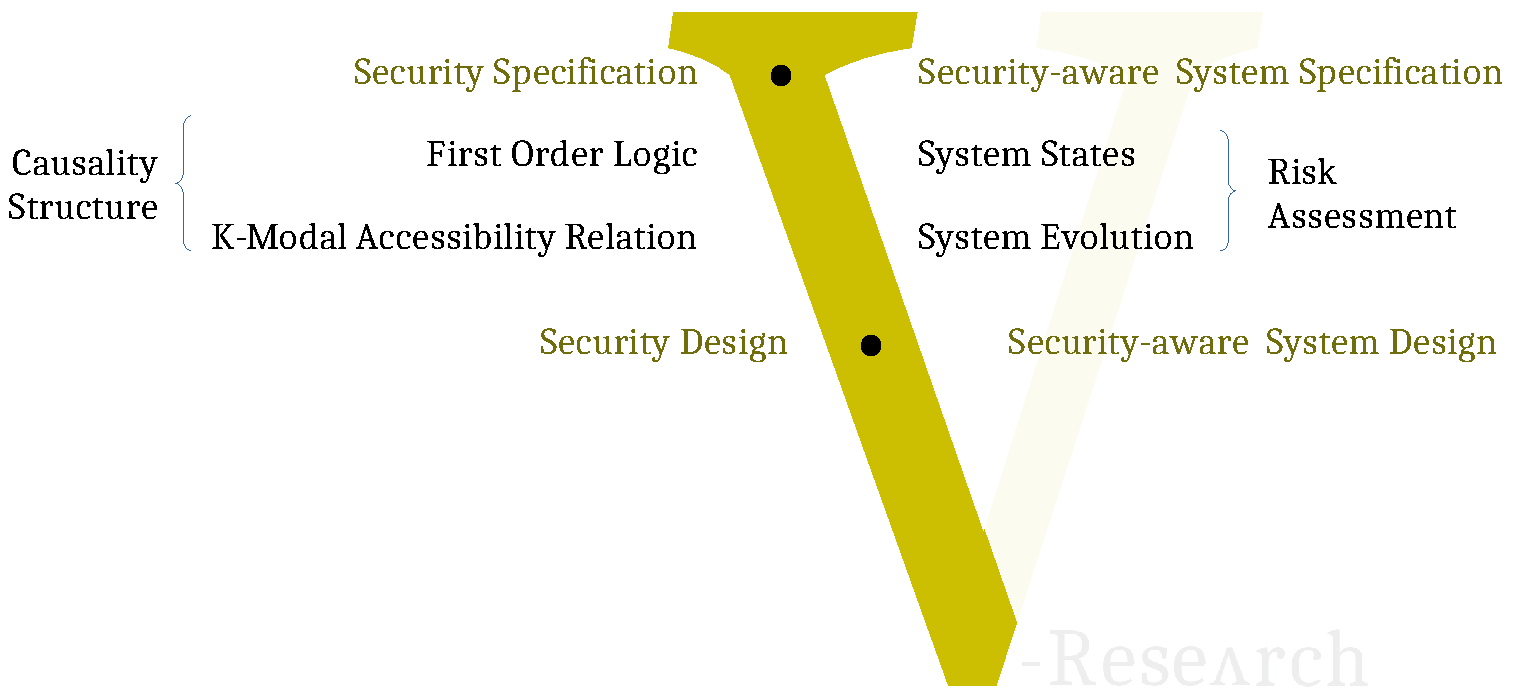
\includegraphics[width=\textwidth]{vmodel.pdf}
	\caption{Cybersecurity Engineering Life-cycle}
	\label{fig:knowledge-belief}
\end{figure}

Infosec, or Information Security, aims at mitigating the security risks related
to information. The standard de-facto is the so called CIA triad 
(where CIA stands for Confidentiality, Integrity, Availability), which is often
criticized for being too general or non-adequate (e.g. by adding authenticity which is 
often used as a building block for confidentiality and integrity) 
to be effectively applied to the engineering of systems. Due to this,
many researchers an organization tried to improve the CIA triad. 
The evolutions/extensions of the CIA triad has been documented, e.g.,
in \autocite{Samonas2014cia} and is summarized in Table~\ref{tab:ciaevolution}.

\begin{table}[h]
\centering
%\setlength{\tabcolsep}{3.5pt}
%\renewcommand{\arraystretch}{1}
\small
\begin{tabular}{rll} 
	{\bf Year} & {\bf Definition} & {\bf Legend}\\
	\hline
	1970s & infosec = CIA & Confidentiality, Integrity, Availability\\
	1980s & infosec += (Au, nR) & Authenticity and non-Repudiation\\
	1990s & infosec += CSpec & Correctness in Specification\\
	2000s & infosec += RITE & Responsibility, Integrity of people, Trust, Ethicality
\end{tabular}
\caption{Chronological progression of the CIA triad~\label{tab:ciaevolution}}
\end{table}


An example is the effort made by the OECD (Organisation for Economic
Co-operation and Development) in \autocite{OECD2013guidelines} to define
security guidelines for information system (1992) based on new principles such
as ``awareness, ethics, risk assessment'' and maintain those revising the
document (e.g.  following the multistakeholder expert consultation in 2013).
Other similar efforts focused on defining entirely new principles or extending
the CIA triad, such as \autocite{NISTSP800-160}. What is of interest for our
argument is that, to the best of our knowledge, all of the approaches that aim
at improving the CIA triad motivated by empirical evidences. On the contrary,
we now define (in Section~\ref{sec:properties}) the CIA triad for an agent
defined in the $\abftheory$ theory and we test if (i) other properties are
allowed in the $\abftheory$ theory, and (ii) if and how the CIA triad can be
detailed in the $\abftheory$ theory.

\subsection{Elicitation of Security Requirements}\label{sec:properties}
In \autocite{Anderson1972report,Samonas2014cia}, CIA are defined as follows.
\begin{itemize}
	\item Unauthorized information release: an unauthorized person is able
		to read and take  advantage  of  information  stored  in  the
		computer.  This  category of concern  sometimes  extends  to
		``traffic  analysis,''  in  which  the intruder  only observes
		the  patterns  of  information  use.  From  those patterns,
		the  intruder can   infer   some   information   content.
		This category   also   includes   the unauthorized use of a
		proprietary program.  (Confidentiality or Secrecy) 
	\item Unauthorized  information  modification:  an  unauthorized person
		is  able  to make changes in stored information -- a form  of
		sabotage.  It should be noted that in the case of this kind of
		violation, the intruder does not necessarily see the
		information he has changed.  (Integrity)
	\item Unauthorized  denial  of  use:  an  intruder  can  prevent  an
		authorized  user  from referring to, or from modifying
		information, even though the intruder may not be able to refer
		to, neither modify the information themselves. (Availability)
\end{itemize}

We now want to generalize the CIA triad to agents and not just 
information and map it to the $\abftheory$ theory.
\begin{definition}{\bf Infosec-Confidentiality --}\label{def:infosec-c}
	An Information $\varphi$ is considered to be confidential to a set of 
	agents $Ag_c$ if, per each agent $a\in Ag_c$, the content of the
	information (i.e. the data it carries) can only be understood (i.e. the relation
	between the information and its data can be known) by the
	agents in $Ag_c$.

	\begin{itemize}
		\item[$(\interpretation21)$] for all agents $a\in Ag$,
			$\world\models\information{a}{\varphi}$ and
			$\world\models\rcc(\varphi,Conf) \wedge
			\neg\dr{Conf}{\varphi}$ iff for any world $\world'$
			such that $\world \modalrelation\world'$,
			$\world'\models\believe{a}{\varphi}$, and
			$\world'\models\knows{a}{\exists f.~
			f(\information{a}{\varphi})=\varphi}$, where 
			$Conf$ is a Region and $f$ is an uninterpreted function.
	\end{itemize}
\end{definition}

\begin{example}{Dummy security protocol --}
	The last part (part III) of the protocol in our first example
	(Figure~\ref{fig:protocol-example}) represents the actual key exchange
	which, in general, needs to be confidential; otherwise the key would be
	known by any other agent who can, e.g., read on the communication
	channel.  Therefore, the last message, in Alice-and-Bob notation can be
	rephrased as: \begin{displaymath} Alice\Rightarrow Bob: enc(pk(Bob),
	symmetricKey) \end{displaymath} where $enc$ is the standard asymmetric
	encryption operator that encrypts the message $symmetricKey$ with the
	public key of Bob $pk(Bob)$ (see, e.g.,
	\autocite{Rocchetto2017interpolation} for a detailed formalization).
	The function $f$ in Definition~\ref{def:infosec-c}, represents any
	function used to enforce confidentiality on information.  In this
	example, $f$ is identified with $enc$ (i.e.
	$enc(pvt(Bob),symmetricKey)=symmetricKey$), the information is
	$\information{Alice}{[enc(pk(Bob),symmetricKey)]}$ and the data, i.e.
	$\varphi$ in Definition~\ref{def:infosec-c}, is $\varphi=symmetricKey$.
	In the perfect cryptography assumption, and assuming for simplicity
	that the logic of the whole protocol preserves confidentiality, the
	message is confidential. In fact, if $Ag={Alice, Bob}$ and $\eq{symmetricKey}{Conf}$:
	\begin{align*}
		\world^0\models\belief{Alice}{symmetricKey},\\
		\world^1\models\information{Alice}{symmetricKey}, \text{and}\\
		\world^2\models\belief{Bob}{symmetricKey} ~\text{if} \\
		enc(pvt(Bob), \information{Alice}{symmetricKey}=symmetricKey)=symmetricKey\\
		(i.e. f=enc ~\text{and}~ \information{Alice}{symmetricKey}=enc(pub(Bob),symmetricKey))\\
	\end{align*}
\end{example}

\begin{definition}{\bf Agent-Confidentiality --}\label{def:confidentiality}
An agent preserves the property of confidentiality iff 
\end{definition}

\begin{definition}{\bf System-Confidentiality --}\label{def:confidentiality}
	The property of confidentiality holds in a system when its information
	preserves confidentiality.
\end{definition}


\fix{mr}{
Confidentiality: the information is accessible only to authorised individuals.
A set of rules that limits access to information.  The information can be
accessed by X if and only if X is authorized to access it = X has the right
attributes (i.e. keys, password) to access it.

Integrity: the information is trustworthy and accurate (i.e. uncorrupted and
unaltered). Protects data from modification or deletion by unauthorized sources
and the ability to undo any damage done.  (for data at rest) If the information
X is written, A will always be read. If information X is modified to
information X', information X can always be recovered.  (for data in transit)
If the information X is sent, A will be received. If information X is modified
to information X', information X can always be recovered.

Availability: the information is accessible and usable when required. Guarantee
of reliable access to the information by authorized people If the information X
needs to be accessed, information X can be retrieved. If

Authenticity: assurance that the information is from the source it claims to be
from. Authenticity involves proof of identity. Authenticity is verified through
authentication.  If information X arrives from A to B, A sent information X and
B can verify it.  ??Authenticity implies integrity but Integrity doesn't imply
authenticity??  ??Authenticity doesn't imply confidentiality but
confidentiality does imply authenticity??

Non-repudiation: the ability to ensure that a party to a contract or a
communication cannot deny the authenticity of their signature on information
(or the sending of) that they originated.  If information X arrives from A, A
sent it and cannot deny it (partial overlap??).  If sender A sends information
X, it cannot say he didn't do it.  Non-repudiation implies authenticity and
integrity. Authenticity doesn't imply non-repudiation (replay attacks?).
Integrity doesn't imply non-repudiation (replay attacks?). 
}

\subsubsection{Relevant Standards}\label{sec:standards}
\begin{enumerate}[noitemsep]
	\item DO-326A
\end{enumerate}

\begin{enumerate}
\item specification -- definition of the desired design of a system. The
specification is verified w.r.t. the  $\abf$ theory. Checking the
controls of the whole cybersecurity life-cycle and the relation with
CWE.
\item design -- the mitigations identified in the specification stage
are implemented into the design. The security of the assets w.r.t. the design are
verified with a, so called, cybersecurity risk assessment.
\end{enumerate}


\section{Prototype and Empirical Tests}\label{sec:prototest}
\subsection{Prototype Implementation}\label{sec:tool}
\subsection{Empirical Tests}\label{sec:tests}

\section{Conclusion and Related Work}\label{sec:related}

\printbibliography

\end{document}
